% This is sigproc-sp.tex -FILE FOR V2.6SP OF ACM_PROC_ARTICLE-SP.CLS
% OCTOBER 2002
%
% It is an example file showing how to use the 'acm_proc_article-sp.cls' V2.6SP
% LaTeX2e document class file for Conference Proceedings submissions.
% ----------------------------------------------------------------------------------------------------------------
% This .tex file (and associated .cls V2.6SP) *DOES NOT* produce:
%       1) The Permission Statement
%       2) The Conference (location) Info information
%       3) The Copyright Line with ACM data
%       4) Page numbering
%
%  However, both the CopyrightYear (default to 2002) and the ACM Copyright Data
% (default to X-XXXXX-XX-X/XX/XX) can still be over-ridden by whatever the author
% inserts into the source .tex file.
% e.g.
% \CopyrightYear{2003} will cause 2003 to appear in the copyright line.
% \crdata{0-12345-67-8/90/12} will cause 0-12345-67-8/90/12 to appear in the copyright line.
%
% ---------------------------------------------------------------------------------------------------------------
% It is an example which *does* use the .bib file (from which the .bbl file
% is produced).
% REMEMBER HOWEVER: After having produced the .bbl file,
% and prior to final submission,
% you need to 'insert'  your .bbl file into your source .tex file so as to provide
% ONE 'self-contained' source file.
%
% Questions regarding SIGS should be sent to
% Adrienne Griscti ---> griscti@acm.org
%
% Questions/suggestions regarding the guidelines, .tex and .cls files, etc. to
% Gerald Murray ---> murray@acm.org
%
% For tracking purposes - this is V2.6SP - OCTOBER 2002


% This is sigproc-sp.tex -FILE FOR V2.6SP OF ACM_PROC_ARTICLE-SP.CLS
% OCTOBER 2002
%
% It is an example file showing how to use the 'acm_proc_article-sp.cls' V2.6SP
% LaTeX2e document class file for Conference Proceedings submissions.
% ----------------------------------------------------------------------------------------------------------------
% This .tex file (and associated .cls V2.6SP) *DOES NOT* produce:
%       1) The Permission Statement
%       2) The Conference (location) Info information
%       3) The Copyright Line with ACM data
%       4) Page numbering
%
%  However, both the CopyrightYear (default to 2002) and the ACM Copyright Data
% (default to X-XXXXX-XX-X/XX/XX) can still be over-ridden by whatever the author
% inserts into the source .tex file.
% e.g.
% \CopyrightYear{2003} will cause 2003 to appear in the copyright line.
% \crdata{0-12345-67-8/90/12} will cause 0-12345-67-8/90/12 to appear in the copyright line.
%
% ---------------------------------------------------------------------------------------------------------------
% It is an example which *does* use the .bib file (from which the .bbl file
% is produced).
% REMEMBER HOWEVER: After having produced the .bbl file,
% and prior to final submission,
% you need to 'insert'  your .bbl file into your source .tex file so as to provide
% ONE 'self-contained' source file.
%
% Questions regarding SIGS should be sent to
% Adrienne Griscti ---> griscti@acm.org
%
% Questions/suggestions regarding the guidelines, .tex and .cls files, etc. to
% Gerald Murray ---> murray@acm.org
%
% For tracking purposes - this is V2.6SP - OCTOBER 2002


\documentclass{sig-alternate}

\usepackage{hyperref}
\usepackage{verbatim}


\begin{document}




%
% --- Author Metadata here ---
%\conferenceinfo{WOODSTOCK}{'97 El Paso, Texas USA}
%\setpagenumber{50}
%\CopyrightYear{2002} % Allows default copyright year (2002) to be over-ridden - IF NEED BE.
%\crdata{0-12345-67-8/90/01}  % Allows default copyright data (X-XXXXX-XX-X/XX/XX) to be over-ridden.
% --- End of Author Metadata ---
%\conferenceinfo{PPoPP'05,} {June 15--17, 2005, Chicago, Illinois, USA.}
%\CopyrightYear{2005}
%\crdata{1-59593-080-9/05/0006} 


\title{A Case Study on Matrix-Matrix Multiplication \\ in the Alamode Lab
}
%
% You need the command \numberofauthors to handle the "boxing"
% and alignment of the authors under the title, and to add
% a section for authors number 4 through n.
%
% Up to the first three authors are aligned under the title;
% use the \alignauthor commands below to handle those names
% and affiliations. Add names, affiliations, addresses for
% additional authors as the argument to \additionalauthors;
% these will be set for you without further effort on your
% part as the last section in the body of your article BEFORE
% References or any Appendices.

\numberofauthors{1}
%
% You can go ahead and credit authors number 4+ here;
% their names will appear in a section called
% "Additional Authors" just before the Appendices
% (if there are any) or Bibliography (if there
% aren't)

% Put no more than the first THREE authors in the \author command
\author{
%
% The command \alignauthor (no curly braces needed) should
% precede each author name, affiliation/snail-mail address and
% e-mail address. Additionally, tag each line of
% affiliation/address with \affaddr, and tag the
%% e-mail address with \email.
\alignauthor Brian Hoenes \\
%\titlenote{Dr.~Trovato insisted his name be first.}\\
       \vspace{1mm}
       \affaddr{Department of Electrical Engineering and Computer Sciences}\\
       \affaddr{Colorado School of Mines, Golden, CO 80401, USA}\\
       \email{bhoenes@mines.edu}
}

%\additionalauthors{Additional authors: John Smith (The Th{\o}rv\"{a}ld Group,
%email: {\texttt{jsmith@affiliation.org}}) and Julius P.~Kumquat
%(The Kumquat Consortium, email: {\texttt{jpkumquat@consortium.net}}).}
%\date{30 July 1999}
\maketitle

\begin{abstract}


It has been demonstrated recently that single fail-stop process 
failure in ScaLAPACK matrix multiplication can be tolerated 
without checkpointing. Multiple simultaneous processor failures 
can be tolerated without checkpointing by encoding matrices using 
a real-number erasure correcting code. However, the floating-point 
representation of a real number in today's high performance 
computer architecture introduces round off errors which can 
be enlarged and cause the loss of precision of possibly all 
effective digits during recovery when the number of processors in the system is large.

In this paper, we present a class of Reed-Solomon style 
real-number erasure correcting codes which have optimal 
numerical stability during recovery. We analytically 
construct the numerically best erasure correcting 
codes for 2 erasures and develop an approximation 
method to computationally construct numerically 
good codes for 3 or more erasures. Experimental 
results demonstrate that the proposed codes are 
numerically much more stable than existing codes.



\end{abstract}

% A category with the (minimum) three required fields
%\category{H.4}{Information Systems Applications}{Miscellaneous}
%A category including the fourth, optional field follows...
%\category{D.1.3}{Programming Techniques}{Concurrent Programming}[ Parallel programming ]

%\terms{Design, Reliability, Performance}

%\keywords{Fault Tolerance, High Performance Computing, 
%%Matrix Operations, Numerical Stability, Real-Number Codes, 
%Reed-Solomon Erasure Codes, ScaLAPACK.} % NOT required for Proceedings


\newtheorem{theorem}{Theorem}


\section{Introduction}
\label{sec:intro}


While the peak performance of the contemporary high performance computing (HPC) systems
continues to grow exponentially, it is getting more and more difficult 
for scientific applications to achieve high performance due to both 
the complex architecture of and the increasing failures in these systems.
Schroeder and Gibson from Carnegie Mellon University (CMU) recently studied
the system logs of 22 HPC systems in Los Alamos National Laboratory (LANL)
and found that the mean-time-to-interrupt (MTTI) for these HPC 
systems varies from about half a month to less than half a day~\cite{gibson1:failure, gibson2:failure, gibson3:failure}. 
In order to use these systems efficiently and avoid restarting computations 
from beginning after failures, applications have to be able to tolerate failures.
Today's long running scientific applications typically tolerate failures by 
checkpointing~\cite{cappello:ft, chen:scalable-checkpointing, plank:dc,plank97:rscode, stellner:cocheck, wang:blcr}. 
Checkpointing can usually be used in different type of systems and to 
a wide range of applications. However, when applications modify 
a large amount of memory between two consecutive checkpoints, 
checkpointing often introduces a considerable overhead~\cite{kim96:abft, plank:abft}. 

Matrix operations (such as matrix multiplication, 
solving system of linear equations, and finding eigenvalues and eigenvectors, etc) 
are fundamental operations in science and engineering. Some important 
linear algebra operations such as Gaussian 
elimination have been proved to be able to scale to more than 100,000 
processors and achieve more than one petaflops on today's HPC systems~\cite{top500}. 
However, today's widely used dense linear algebra 
software such as ScaLAPACK~\cite{dongarra96:scalapack} and  PLAPACK~\cite{geijn:plapack}
usually modifies a large amount of memory between  checkpoints, therefore, 
checkpointing techniques often introduce a considerable overhead into the computation.
The high frequency of failures and the large number of processors in the
next generation HPC systems will further exacerbate the problem.

In~\cite{chen:abft}, a highly scalable checkpoint-free techniques was
proposed to tolerate single fail-stop failure in high performance 
matrix operations on large scale HPC systems. It was also 
demonstrated that the overhead rate of this scheme decreases 
with a speed of $1/\sqrt{p}$ when the number of processors $p$ increases. 
However, in order to tolerate multiple simultaneous process failures 
with minimum redundancy, a real number version Reed-Solomon style 
erasure correcting codes have to be used to encode the input matrices. 

In existing Reed-Solomon style real number erasure correcting codes, 
the generator matrices mainly include: Vandermonde 
matrix (Vander)~\cite{hadjicostis:coding}, 
Vandermonde-like matrix for the Chebyshev polynomials 
(Chebvand)~\cite{boley92:abft}, Cauchy matrix (Cauchy), 
Discrete Cosine Transform matrix (DCT), Discrete Fourier 
Transform matrix (DFT)~\cite{Ferreira00, Ferreira03}, Gaussian 
random matrix~\cite{zchen:random_codes, zchen:random_condition},
and Grassmannian frame matrix~\cite{strohmer03:grassmannian}. 
If there is no round-off errors in the representation of a real number, 
these generator matrices can all be used 
as the encoding matrices of the proposed checkpoint-free 
techniques in~\cite{chen:abft}.

However, in today's computer arithmetic where no computation
is exact due to round-off errors, it is well 
known~\cite{golub89:matrix} that, in solving a 
linear system of equations, a condition number of $10^k$ for the coefficient matrix
leads to a loss of accuracy of about $k$ decimal digits in the solution.
The coefficient matrix of the system of equations to be solved during recovery
may be any square sub-matrix (including minor) of the generator matrix.
Therefore, in order to get a numerically good recovery for any erasure patterns, 
{\it any square sub-matrix (including minor) of the generator matrix
has to be well-conditioned.}

But the generator matrices from existing Reed-Solomon style 
real number erasure correcting codes 
mentioned above all contain many ill-conditioned sub-matrices when the sizes
of these generator matrices are large.
Therefore, in these real number codes, when certain erasure patterns occur, 
an ill-conditioned linear system has to be solved to reconstruct
an approximation of the original information, which can cause the 
loss of precision of possibly all digits in the recovered numbers.
To the best of our knowledge, it is still open whether there 
exists any arbitrarily large generator matrix 
that can correct all erasures or not. It is also an open problem how to
find the codes with optimal numerically stability. 

In this paper, we present a class of numerically optimal Reed-Solomon 
style real-number erasure correcting codes.  
We construct the numerically optimal erasure correcting codes for 
two erasures analytically and develop an approximation method to 
approximate the numerically optimal codes for three or more erasures computationally.
We explore the property of generator matrices that are able to correct all erasure patterns.
We prove no minimum redundancy codes can correct all erasure patterns 
when the size of processors is large and the number 
of erasures is more than one. We give an upper bound on 
the number of processors so that all two erasure patterns can be corrected. 
Experimental results demonstrate that our codes are numerically 
much more stable than existing codes. 


Although we only focus on the correcting of erasures in this paper,
it is also possible to use our codes (generator matrices) to correct errors 
through the $l_1$ minimization techniques proposed in~\cite{tao:codes, donoho:L1_minimization}.
While this paper develops the codes for fault tolerant matrix operations, 
the codes can also be used in many other fields such as compressive sensing~\cite{donoho:compressed} and fault tolerant  combinatorial and dynamic systems~\cite{hadjicostis:coding}.


The rest of the paper is organized as following. Section 2 introduces 
techniques for fault tolerant matrix operations.
In Section 3, we explore the numerical properties of existing real number
codes and present a class of real number codes that have optimal numerical stability.
In Section 4, we analytically construct the numerically best erasure 
correcting codes for two erasures.
Section 5 develops an approximation method to 
approximate the numerically optimal codes for three 
or more erasures computationally.
In Section 6, we compare various real number codes experimentally.
Section 7 concludes the paper and discusses the future work.


\section{ Fault Tolerant Matrix Operations}

Matrix operations are fundamental for science and engineering.
Incorporating fault tolerance into matrix operations 
has been extensively studied for many years by many researchers~\cite{anfinson:abft, 
Banerjee90:abft, Balasubramanian90:abft, boley92:abft,  
zchen:random_codes, zchen:random_condition, chen:abft, chen:scalable-checkpointing, 
gunnels:abft, huang84:abft, kim96:abft, langou:ft, luk84:abft, 
plank:abft, redinbo2:abft, redinbo:abft, wang:abft}.

In~\cite{huang84:abft}, the algorithm based fault tolerance (ABFT) is proposed to 
detect, locate, and correct miscalculations. The idea is to encode 
the original matrices using real number codes and then re-design 
algorithms to operate on the encoded matrices. In~\cite{huang84:abft}, 
Huang and Abraham proved
that the encoding relationship in the input encoded  matrices 
is preserved \textit{\bf  at the end of the computation 
no matter which algorithm is used} to perform the computation.
Therefore, processor miscalculations can be detected, 
located, and corrected at the end of the computation.
ABFT researches have mostly focused on detecting, locating, 
and correcting miscalculations or data corruption where failed processors are 
often assumed to be able to continue their work
but produce incorrect calculations or corrupted data. The error detection are
often performed at the end of the computation by checking whether the 
final computation results satisfy the encoding relationship or not.

However, in a distributed environment, if a failed processor stops working,
then we need to be able to detect, locate, and recover the data 
{\bf in the middle of the computation}.
In order to be able to recover in the middle of the computation, 
a global consistent state of the application is often required. 
Checkpointing and message logging are typical approaches to 
maintain or construct such a global consistent state. 
In~\cite{ chen:scalable-checkpointing, 
zchen05:diskless, zchen05:ft-mpi, zchen:dissertation, kim96:abft},
real number erasure correcting codes are used to 
encode the checkpoint data to maintain a global consistent state
with redundancy periodically. 


Recently, in~\cite{chen:abft}, it has been demonstrated that 
fault tolerance (for fail-stop failures) for 
large scale parallel matrix operations on today's
large HPC systems can be achieved without 
any checkpointing (or message logging)
by encoding the original matrices into 
larger weighted checksum matrices
using real-number erasure correcting codes. 
The scheme is highly scalable with low overhead. 
The overhead rate decreases with a speed of $1/\sqrt{p}$ 
when the number of processors $p$ increases. 


Traditional erasure correcting codes based on finite fields do 
{\bf NOT} work~\cite{zchen:random_codes}
for the techniques in~\cite{huang84:abft, chen:abft}. 
Real number codes have to be used to encode the input matrices.
In order to be able to recover from multiple simultaneous failures of any patterns, 
the encoding matrix have to be chosen very carefully. 
This encoding matrix is often called the generator 
matrix of a linear code in coding theory. 
The goal of this paper is to find an appropriate
generator matrix to encode the input matrices
so that multiple simultaneous failures in 
large scale parallel matrix operations can be recovered
without any checkpointing (or message logging).



\section{Real-Number Codes for Fault Tolerant Matrix Operations}


The research on real number codes can be dated back to~\cite{marshall:realcodes}. Recently,
codes based on random matrices~\cite{zchen:random_codes_utk, zchen:random_codes, zchen:random_condition} 
and Grassmannian frames~\cite{goyal: erasure, strohmer03:grassmannian} have been proposed to 
improve the numerically stability of the recovery.
However, it is still an open problem what is the numerically best real number codes. 
In this section, we discuss some popular real number codes and propose
a class of new real number codes which have optimal numerical stability. 

Let $ x = ( x_1, x_2, . . ., x_n )^T \in \mathcal{R}^n $ 
denote the original information, and $ G_{m \times n} $ denote a $m$ by $n$ real number matrix.
The redundant information $c = ( c_1, c_2, . . ., c_m)^T \in \mathcal{R}^m $
is calculated by
\begin{equation}
\label{eq2}
\begin{cases}
g_{1 1} x_1 + \ldots + g_{1 n} x_n & =   c_1 \\
& \vdots   \\
g_{m 1} x_1 + \ldots + g_{m n} x_n & =   c_m. 
\end{cases}
\end{equation}

$G_{m \times n}$  is often called the generator matrix of the linear code.
We also call $G_{m \times n}$ the encoding matrix for fault tolerant matrix 
operations. In a fault tolerant matrix operations, the original 
information $x_i$ is the local matrix in the local memory of a processor. 
Without loss of generality and for the simplicity of the discussion, 
in this paper, we assume $x_i$ is just a real number.

The relationship in (1) actually
establishes $m$ equalities between the original data $x$ 
and the redundant information $c$.
If $k$ (where $k\leq m$) elements of $x$ are erased,
then the $m$ equalities 
become a system of linear equations with $k$ unknowns.
When the generator $G_{m \times n}$ is appropriately chosen, 
the lost $k$ elements in $x$ can be able to be reconstructed through 
solving this system of linear equations with $k$ unknowns.


The real number coding theory problem we want to solve is: 
{\it how to choose the generator matrix $G_{m \times n}$ in~(1),
such that, after any no more than $m$ erasures in $x$,
a good approximation of all erased elements in
$x$ can still be reconstructed by solving the system of linear equations 
derived from (1)?}


\subsection{Real-Number Codes Derived from Finite Field Codes}
In~\cite{Nair90}, Nair and Abraham proved that, for any finite field code,
there is a corresponding code in real number field.
In the existing codes derived from finite fields,
the generator matrices mainly include: Vandermonde matrix (Vander)~\cite{hadjicostis:coding}, 
Vandermonde-like matrix for the Chebyshev polynomials (Chebvand)~\cite{boley92:abft} 
Cauchy matrix (Cauchy), Discrete Cosine Transform matrix (DCT), and  
Discrete Fourier Transform matrix (DFT)~\cite{Ferreira00, Ferreira03}. These generator
matrices all contain many ill-conditioned sub-matrices 
when the size the generator matrices become large. Therefore, in these codes, when
certain erasure patterns occur, an ill-conditioned linear system of equations has to be solved
to reconstruct an approximation of the original information, which can cause
the loss of precision of possibly all digits in the recovered numbers.



\subsection{Real-Number Codes Based on Random Matrices}

In~\cite{zchen:random_codes_utk, zchen:random_codes, zchen:random_condition},  
Gaussian and uniform random matrices have been proposed as the encoding (generator) matrices.
It is well know that Gaussian random matrices are well conditioned~\cite{edelman88:randm}.
Note that any sub-matrix of a Gaussian random matrix is still a Gaussian random matrix,
therefore, Gaussian random matrix can guarantee the recovery of the lost data with high probability.

 
\subsection{Real-Number Codes Based on Grassmannian Frames}

While Gaussian random codes is good with high probability, it is nondeterministic.
It has been shown in~\cite{knuth:random} that Gaussian random distribution 
in $\mathcal{R}^n$ is equivalent to uniform random distribution in the unit sphere
$\mathcal{S}^{n-1}$ of $\mathcal{R}^n$.
Uniformly distributed points on hyper spheres tend to maximize 
the minimum sphere distance between points.
If the sphere distance of two points is zero, 
the corresponding two columns of the matrix are the same. 
The sub-matrices containing these two columns are singular.
When two vectors are the same, the correlation of the two vectors
is 1. The Grassmannian frame idea minimize the maximum correlations 
between columns of the generator matrices~\cite{goyal: erasure, strohmer03:grassmannian}.

A sequence of vectors $\{g_k\}_{k=1}^{n} \in \mathcal{R}^m$ 
is called a Grassmannian frame if it is the solution to
\begin{eqnarray} 
\displaystyle \min_{\{f_k\}_{k=1}^{n} \in \mathcal{R}^m, < f_k, f_k > = 1 }
\left\{ \displaystyle \max_{i \neq j} \left\{  < f_i, f_j > \right\}  \right\}
\end{eqnarray} 

The Grassmannian frame code is defined as the 
code whose generator matrix is $G_{m \times n} = (g_1, g_2, \ldots, g_n)$.

Minimizing the maximum correlations is equivalent to maximizing 
the minimum angle between columns of the generator matrices. 
The problem of maximizing the minimum angle between vectors on a hyper sphere
is called the Grassmannian (line) packing problem~\cite{conway:grassmannian}. 
It is hard to find optimal arrangements of points even on a 2-sphere (i.e. $m=3$).
Steve Smale has listed the problem of "distribution of points on the 2-sphere" 
as the problem $\#7$ of a total of 18 unsolved mathematics 
problems in twenty-first century~\cite{smale:unsolved}.
There are no general analytical solutions for this 
problem except for some special combinations of 
$m$ and $n$~\cite{grass}.



\subsection{Real-Number Codes with Optimal Numerical Stability}

The Grassmannian frame code minimizes the maximum correlations 
between columns of the generator matrices, however, the accuracy during recovery is 
directly related only to the condition number of the equations to be solved and condition number
is a property that associated with more than two columns of a matrix. 
Even if the maximum correlations are minimized, it is still possible 
that the generator matrix contains a singular sub-matrix. Therefore,
in order to get better codes, we decide to work on minimizing the maximum condition numbers
of sub-matrices of a generator matrix directly.

The recovery procedure involves solving a system of linear equations
with one of the sub-matrices from the generator matrix $G$ as the coefficient matrix. 
The coefficient matrix can be any sub-matrix including minor
of $G$. It is well known that in order to get a numerically good solution,
the coefficient matrix has to be well conditioned. Therefore, in order
to be able to recover from all erasure patterns, the generator matrix $G$
has to satisfy any square sub-matrix including minor of $G$ have to be well conditioned. 

If the worst conditioned sub-matrix of $G$ is well conditioned, 
then all the sub-matriices of $G$ will be well conditioned. 
Therefore, we look for generator matrices $G$ for which the 
condition number of the worst conditioned sub-matrix is minimized.  

There are finite number of square sub-matrices in $G$, therefore, we can rank 
these sub-matrices. Let $G_i$ denote the $i^{th}$ square sub-matrix of $G$, 
then the matrix $G^*$ that minimizes the condition number of the worst conditioned square sub-matrix of $G$
is the solution of the following minimax problem.
\begin{eqnarray} 
f(m,n)=\displaystyle \min_{ G_{m \times n} \in \mathcal{R}^{m \times n} }
\left\{  \displaystyle \max_{i} \left\{ \kappa (G_i) \right\}  \right\}
\end{eqnarray} 



The code $G^*$ obtained from the solution of the above minimax problem (3)
is numerically best in the sense that the generator matrix  obtained
has the condition number of the worst conditioned sub-matrix minimized. 
$f(m,n)$ is the condition number of the worst conditioned sub-matrix of the 
optimal $G^*$ obtained. It is well known~\cite{golub89:matrix} that, in solving 
a linear system of equations, a condition number of $10^k$ for the coefficient matrix
leads to a loss of accuracy of about $k$ decimal digits in the solution. 
Therefore, $f(m,n)$ can be used to estimate
the worst case recovery accuracy. For example in IEEE standard 754  
floating point numbers, there are 16 digits of accuracy. 
Then the worst case recovery can guarantee an accuracy 
of  $16 - \log_{10} f(m, n) $ digits. 

The minimax problem specified in (3) is also difficult even if $G$ is restricted 
on matrices with unit norm columns. Actually, when G is restricted 
on matrices with unit norm columns, the problem also becomes finding optimal arrangements of
points on hyper-sphere. As we discussed before in Section 3.3, 
it is an open mathematical problem to
find optimal arrangements of points even on a 2-sphere~\cite{smale:unsolved}.



\section{ Optimal Real-Number Codes for Two Erasures}
In what follows we will solve problem (3)  for the special case when $m=2$.
The generator matrices we obtain is the generator matrices for 
numerically best real-number codes for two erasures.
$f(2,n)$ we obtain is the condition number of the worst conditioned sub-matrix
of the numerically best real-number codes for two erasures.

If there are elements with value zero in the generator matrix, there will be 
singular $1 \times 1$ sub-matrices in the generator matrix.
Therefore, when solving (3), we just need to consider generator matrices
with none of their elements being $0$. Without loss of generality, we assume the
elements of $G$ is non-zero.  When $m=2$, it is enough to just consider
all the $2 \times 2$ sub-matrices.

For any $2 \times n$ matrix $ G_{2 \times n} \in \mathcal{R}^{2 \times n} $, 
let $g_j$ denote the $j^{th}$ column of $G_{2 \times n}$.
Let $G_{ij}$ denote the sub-matrix of $G_{2 \times n}$ consisting
of the column $i$ and $j$ of $G_{2 \times n}$. 
\begin{theorem}
Let 
\begin{eqnarray}
f(2,n)=\displaystyle \min_{ G_{2 \times n} \in \mathcal{R}^{2 \times n} } 
\left\{ \displaystyle \max_{i,j} \left\{  \kappa (G_{ij}) \right\}  \right\}
\end{eqnarray}
Then, 
\begin{eqnarray}
f(2,n)
&=& \sqrt {\frac{1 + \cos \frac{\pi}  {n} }
{1- \cos \frac{\pi}  {n} } }
\end{eqnarray}
The following generator matrix is one of the solutions for (4)
\[ G= \left( \begin{array}{cccc}
\cos\frac{\pi}{2n}&\cos\frac{3\pi}{2n}&\ldots&\frac{(2n-1)\pi}{2n}  \\
\sin\frac{\pi}{2n}&\cos\frac{3\pi}{2n}&\ldots&\frac{(2n-1)\pi}{2n}      \end{array} \right)\]
\end{theorem}

\begin{proof}
\begin{figure}
\centering
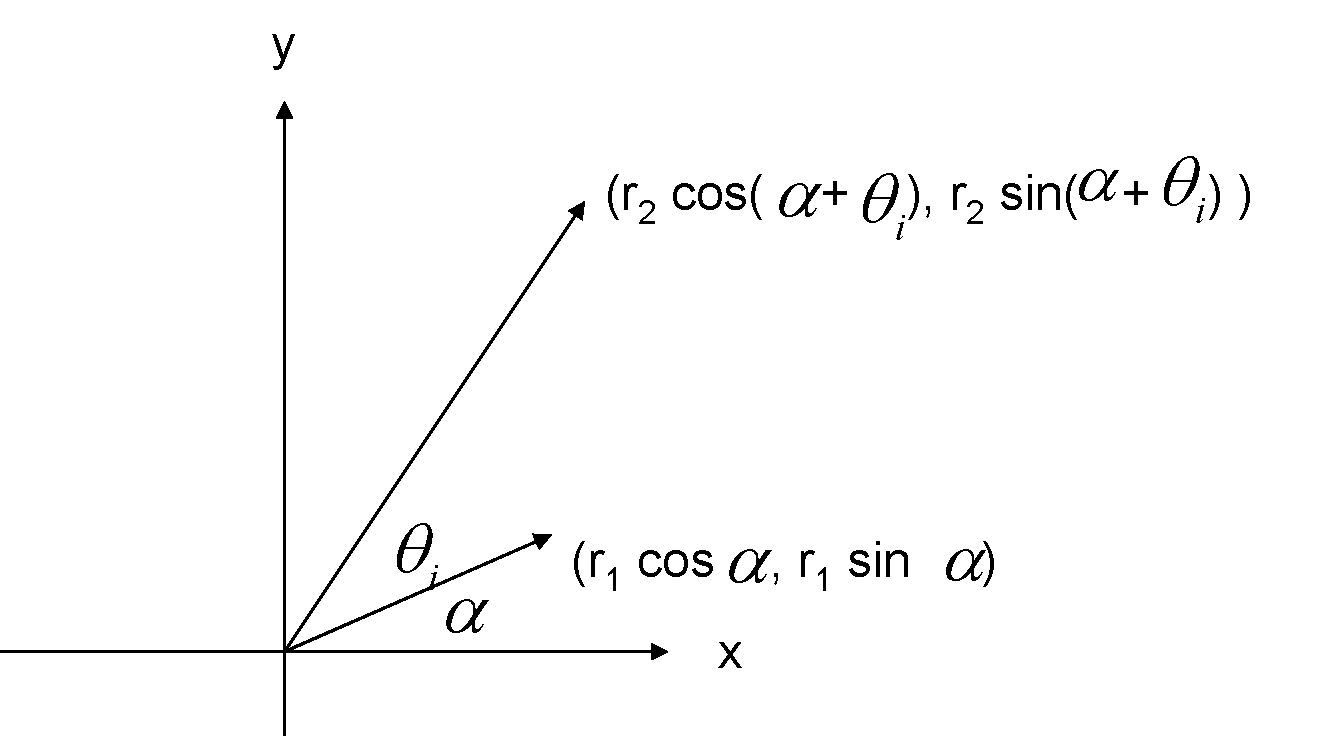
\includegraphics[width=3in]{opt_2erasures.png}
\caption{Polar coordinate representation for a sub-matrix}
\label{polar}
\end{figure}

In a polar coordinate system (Figure 1), the $i^{th}$ column of $G_{2 \times n}$ can be represented as
\[ g_j= \left( \begin{array}{c}
r_i \cos \theta_i  \\
r_i \sin \theta_i  \end{array} \right)\]
$ G_{2 \times n} $ can be represented as 
\[ G_{2 \times n} = \left( \begin{array}{ccc}
r_1 \cos \theta_1 & \ldots & r_n \cos \theta_n \\
r_1 \sin \theta_1 & \ldots & r_n \sin \theta_n    \end{array} \right)\]
$G_{i,j}$ can be represented as 
\[ G_{ij}= \left( \begin{array}{cc}
r_i \cos \theta_1 & r_j \cos \theta_j \\
r_i \sin \theta_1 & r_j \sin \theta_j    \end{array} \right)\]

Therefore,
\[ G_{ij}^T G_{ij}= \left( \begin{array}{cc}
r_i^2 & r_i r_j \cos (\theta_j- \theta_i) \\
r_i r_j \cos (\theta_j- \theta_i) &   r_j^2  \end{array} \right)\]

Note that $G_{ij}^T G_{ij}$ is symmetric and positive definite,
therefore, all its eigenvalues are positive real numbers.
Let $\lambda_{max} (G_{ij}^{T} G_{ij})$ denote the maximum eigenvalue
of $G_{ij}^{T} G_{ij}$ and $\lambda_{min} (G_{ij}^{T} G_{ij})$ denote 
the minimum eigenvalue of $G_{ij}^{T} G_{ij}$, then
\begin{eqnarray*}
\lambda_{max} (G_{ij}^{T} G_{ij})
&=& \frac{ r_{i}^2 + r_{j}^2}{2 } + \\
& &   \sqrt { \frac{ (r_{i}^2 + r_{j}^2)^2}{2^2 } + 
r_{i}^2 r_{j}^2 (\cos (\theta_j - \theta_i)  -1 )}
\end{eqnarray*}
\begin{eqnarray*}
\lambda_{min} (G_{ij}^{T} G_{ij})
&=& \frac{ r_{i}^2 + r_{j}^2}{2 } - \\
& &  \sqrt { \frac{ (r_{i}^2 + r_{j}^2)^2}{2^2 } + 
r_{i}^2 r_{j}^2 (\cos (\theta_j - \theta_i)  -1 )}
\end{eqnarray*}

Therefore,
\begin{eqnarray}
\kappa (G_{ij}) \nonumber
&=& \sqrt {\frac {\lambda_{max} (G_{ij}^{T} G_{ij})}
 {\lambda_{min} (G_{ij}^{T} G_{ij})} } \\ \nonumber
&=& \sqrt { \frac {1 + \sqrt {1+\frac{4(\cos^2 (\theta_j -\theta_i)  -1)}
{ \left( \frac{r_{i}}{r_{j}}+\frac{r_{j}}{r_{i}}  \right)^2     }  } }
{1 - \sqrt {1+\frac{4(\cos^2 (\theta_j -\theta_i)  -1)}
{ \left( \frac{r_{i}}{r_{j}}+\frac{r_{j}}{r_{i}}  \right)^2   } } }
}  \\ 
&\geq&  \sqrt { \frac {1 + \sqrt {1+\frac{4(\cos^2 (\theta_j -\theta_i)  -1)}
{ \left( 2 \sqrt { \frac{r_{i}}{r_{j}} \frac{r_{j}}{r_{i}} } \right)^2     }  } }
{1 - \sqrt {1+\frac{4(\cos^2 (\theta_j -\theta_i)  -1)}
{ \left( 2 \sqrt { \frac{r_{i}}{r_{j}} \frac{r_{j}}{r_{i}} } \right)^2   } } }
}    \\ \nonumber
&=& \sqrt { \frac{1+ |\cos (\theta_j -\theta_i)  | }
{1- |\cos (\theta_j -\theta_i) | }  }
\end{eqnarray}

The equality in (6) {\bf is achieved} when $r_i=r_j$.

Note that the relationship (6) is for any $2 \times 2$ sub-matrix of 
$G_{2 \times n}$, therefore, the $G_{2 \times n}$ that solve
problem (4) has to satisfy $r_1=r_2=\ldots=r_n=r$. Note that
for any matrix $M$, $\kappa(M)=\kappa(r M)$, therefore, during the computation of $f(2,n)$, 
it is enough to just consider $G_{2 \times n}$ whose $r_1=r_2=\ldots=r_n=1$. 

When $r_1=r_2=\ldots=r_n=1$, columns of $G_{2 \times n}$ can be treated 
as vectors on a unit circle centered at (0,0). 
If there is a vector $g_j$ for which the angle $(\theta_j -\theta_1)$ 
is larger than $\pi$ (see $g_j$ in Figure 2), then
there is a vector $g=-g_j$ for which the angle $(\theta -\theta_1)$
is less than $\pi$ and $|\cos (\theta_j -\theta_1)| = |\cos (\theta -\theta_1)|$.
Therefore, it is enough to just consider $G_{2 \times n}$  for which the angle 
between $g_1$ and any other $g_j$ is less than $\pi$ during the calculation
of $f(2,m)$. Without affecting the calculation of $f(2,m)$, 
the columns of $G_{2 \times n}$ can be exchanged
so that the angle between $g_1$ and $g_j$ increases as $j$ increases
(see Figure 3 for such an arrangement). Let $\delta_i$ denote the angle
between the newly re-arranged $g_i$ and $g_{i+1}$ for $i=1,2,\ldots,n-1$ and 
$\delta_n$ denote the angle between $g_n$ and $-g_1$, then
\begin{eqnarray}
\delta_1 + \delta_2 + \ldots + \delta_n=\frac{\pi}{2}
\end{eqnarray}
\begin{figure}
\centering
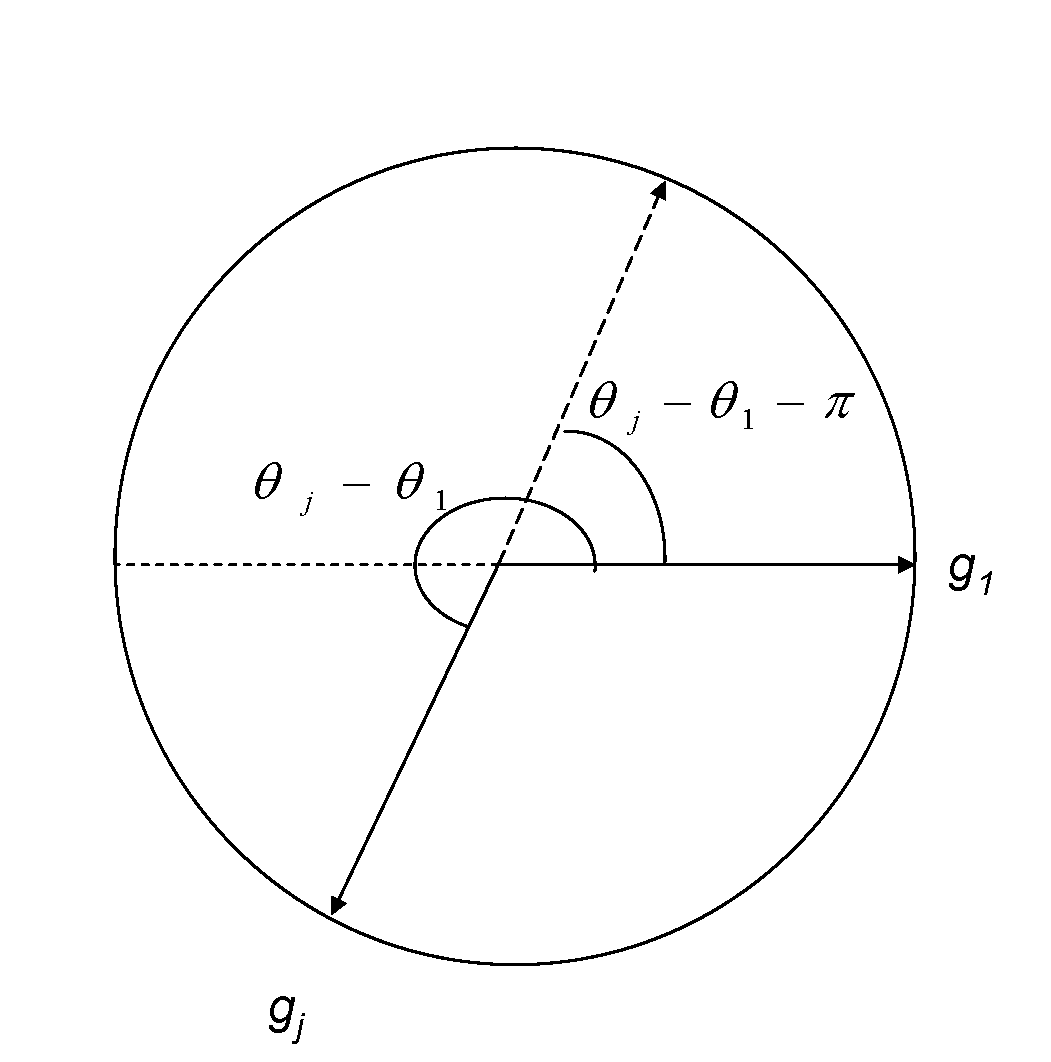
\includegraphics[width=2in]{opt_2erasures_results.png}
\caption{If $(\theta_j -\theta_1)$ is larger than $\pi$, 
then there is a vector $g=-g_j$ for which the angle $(\theta -\theta_1)$
is less than $\pi$ and $|\cos (\theta_j -\theta_1)| = |\cos (\theta -\theta_1)|$.}
\label{spherical ball}
\end{figure}
\begin{figure}
\centering
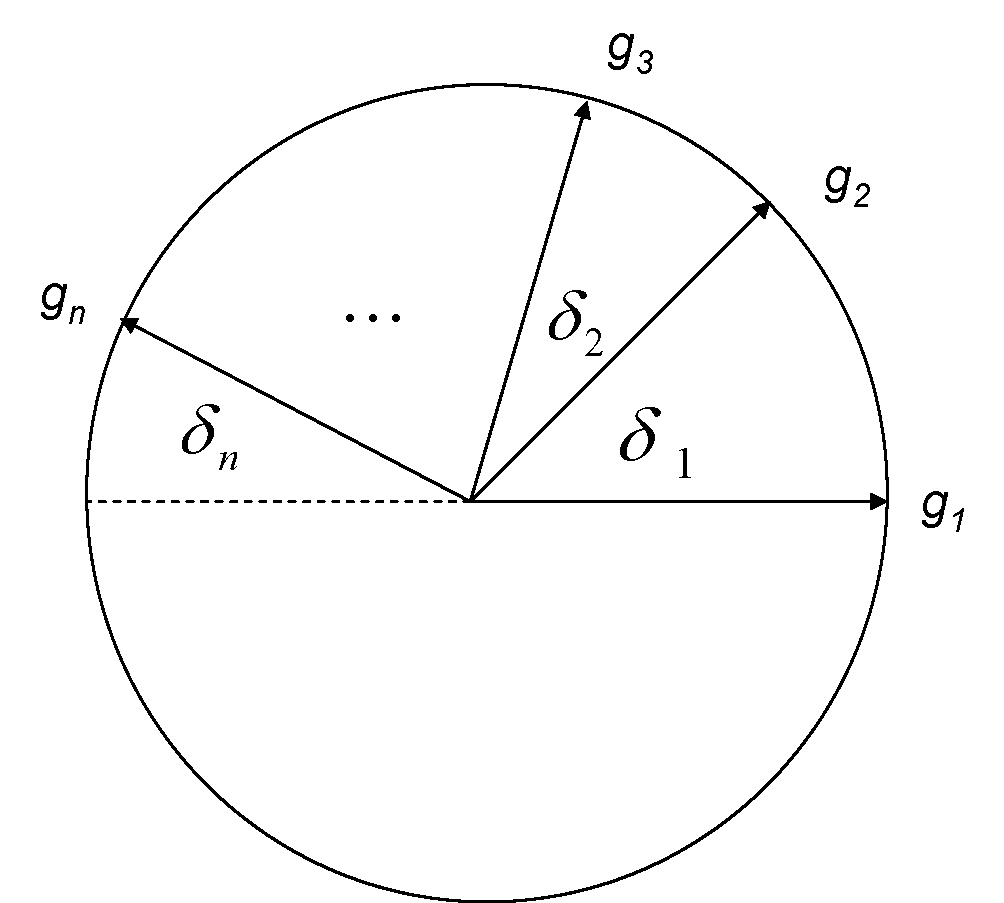
\includegraphics[width=2in]{opt_2erasures_angle.png}
\caption{Adjust columns of $G$ such that $\delta_1 + \delta_2 + \ldots + \delta_n = \frac{\pi}{2}$.}
\label{spherical ball}
\end{figure}


The angle between $g_i$ and $g_j$ is 
\begin{eqnarray}
\theta_j-\theta_i = \delta_i + \ldots + \delta_{j-1}
\end{eqnarray}

Therefore,
\begin{eqnarray}
f(2,n)  \nonumber
&=& \displaystyle \min_{G_{2 \times n} } 
\{ \displaystyle \max_{ij} \{ \kappa (G_{ij} )  \} \} \\ \nonumber
&=& \displaystyle \min_{ r_1=\ldots=r_n=1  }  
\{ \displaystyle \max_{ij} \{ \kappa (G_{ij} ) \} \}  \\ \nonumber
&=& \displaystyle \min_{\delta_1, \ldots, \delta_n} \left \{
\displaystyle \max_{i} \left \{ \sqrt { \frac{1+ |\cos (\theta_j-\theta_i) | }
{1- |\cos (\theta_j-\theta_i) | }  }  \right \} \right \} \\ \nonumber
&=& \displaystyle \min_{\delta_1, \ldots, \delta_n} \left \{
 \sqrt { \frac{1+ |\cos (\displaystyle\min_i \{\delta_i\})  | }
{1- |\cos (\displaystyle\min_i \{\delta_i\} ) | }  }   \right \} \\
&\geq& \displaystyle \min_{\delta_1, \ldots, \delta_n} \left \{
 \sqrt { \frac{1+ |\cos (\frac{\sum_i^n {\delta_i}}  {n} )  | }
{1- |\cos (\frac{\sum_i^n {\delta_i}}  {n} )   | }  }  \right \} \\
&=& \sqrt {\frac{1+ \cos ( \frac{\pi}  {n}  ) }
{1- \cos(  \frac{\pi}  {n}    ) }} 
\end{eqnarray}

The equality in (9) {\bf is achieved}  when 
\begin{eqnarray}
\delta_1=\delta_2=\ldots=\delta_n=\frac{\pi}{n}.
\end{eqnarray}


There is infinite number of optimal $2 \times n$ matrices (codes) with non-zero elements
that satisfy (11). 

The following is a sample optimal $2 \times n$ matrix 
(i.e. a sample numerically best real number erasure correcting code for 2 erasures)
\[ G= \left( \begin{array}{cccc}
\cos\frac{\pi}{2n}&\cos\frac{3\pi}{2n}&\ldots&\frac{(2n-1)\pi}{2n}  \\
\sin\frac{\pi}{2n}&\cos\frac{3\pi}{2n}&\ldots&\frac{(2n-1)\pi}{2n}      \end{array} \right)\]
\end{proof}



Note that when $n$ is large,  
\begin{eqnarray*}
f(2,n)
&=& \sqrt {\frac{1 + \cos \frac{\pi}  {n} }
{1- \cos \frac{\pi}  {n} } } \\
&\approx& \frac {2n}{\pi}  
\end{eqnarray*}

Therefore, the condition number of the worst conditioned sub-matrix
of even the numerically best real-number codes increase 
to infinite approximately linearly when the number of original data items (processors) $n$ increases.
It is {\bf impossible} for even the numerically best 2-erasure code to correct {\bf all}
possible 2-erasures when the number of data items (processors) is large.
The introduced numerical errors can be arbitrarily large during recovery when $n$ is arbitrarily large.

In order to  guarantee to correct {\bf ALL} possible 
2-erasures in IEEE standard 754  floating point numbers (16 digits of accuracy)  with $k$ digits of accuracy
the total number of data items (processors) $n$ has to satisfy
\begin{eqnarray}
n \leq 10^{16-k} \times \frac{\pi}{2}
\end{eqnarray}


If $n\geq 10^{16} \times \frac{\pi}{2}$, all 16 digits in the IEEE standard 754 floating point numbers
will be lost. However, this can be avoided by dividing $n$ processors into sub-groups of the size $s$ and encode
the input matrices within each sub-group.
In order to  guarantee to correct all possible 2-erasures with $k$ 
digits of accuracy in each sub-group, the number of processors $s$
in each sub-group has to satisfy
\begin{eqnarray*}
s \leq 10^{16-k} \times \frac{\pi}{2}
\end{eqnarray*}

Therefore, {\bf with the increase of the redundancy information}, we can 
guarantee to correct all possible 2-erasures with $k$ digits of accuracy.

\section{Construct Numerically Good Codes by Unconstraint Optimization}

As discussed in Section 3, it is one of Smale's 18 unsolved mathematic 
problems~\cite{smale:unsolved}
in the twenty-first century to obtain analytical solution for 
the minimax problem specified in (3) even if $m=3$ and $G$ is restricted 
on matrices with unit norm columns. Instead of solving (3) directly,
in this section, we propose to compute approximate solutions of (3) by solving
another unconstrained optimization problem.
We prove that, for $m=2$, the solution obtained by 
solving the new unconstraint optimization problem
is the same as the solution obtained by solving (3) directly.

Inspired by the $m=2$ case, in what follows, we restrict the choice of the generator matrix $G$ within 
matrices whose column $g_j$ satisfy $||g_j||_2=g_j^T g_j=1$, where $j=1,2, \ldots, n$.
We restrict the choice of sub-matrix within $m \times m$ matrices. 

Let $G_j$ denotes the $j^{th} $ $ m \times m$  sub-matrix of $G_{m \times n}$ 
(the order here can be any order one likes). 
Let $\lambda_1 \geq \lambda_2 \geq \ldots \geq \lambda_m $ denotes the $m$ eigenvalues of $G_j^TG_j$, then
$$\det {(G_j^TG_j)} = \prod_{i=1}^m  \lambda_i$$
$$\sum_{i=1}^m \lambda_i = tr(G_j^TG_j)=m$$
$$1 \leq  \lambda_1 < m$$


Therefore,
\begin{eqnarray*}
\det (G_j)
&=& \sqrt {\det ( G_j^T G_j  ) }  \\
&=& \sqrt {\prod_{i=1}^m \lambda_i  }   \\
&=& \sqrt { \frac{\lambda_1 .  \prod_{i=1}^{m-1} \lambda_i }
{\kappa (G_j^T G_j )  }  }       \\
&\leq& \sqrt {\frac{ \left( \frac{\lambda_1 + \sum_{i=1}^{m-1} \lambda_i} {m} \right)^m}  {\kappa (G_j^T G_j )  }  }    \\
&\leq&  \frac{ 2^{\frac{m}{2} }}  {\kappa (G_j) }         
\end{eqnarray*}

On the other hand,
\begin{eqnarray*}
\det (G_j) 
&=& \sqrt {\det ( G_j^T G_j  ) }  \\
&=& \sqrt {\prod_{i=1}^m \lambda_i  }   \\
&\geq& \sqrt { \lambda_m^m }     \\
&\geq& \sqrt { \frac{1}
{\left(\frac{\lambda_1}{\lambda_m} \right)^m}  }  \\
&=&  \frac{1}{\kappa(G_j)^m}         
\end{eqnarray*}

Therefore, for a fixed $m$,
if $\det (G_j)$ is small, then $\kappa (G_j)$ will be large.
if  $\kappa (G_j)$  is large, then  $\det (G_j)$ will be small.



Note that,
\begin{eqnarray*}
\det ( G_j ) 
&=& \sqrt {\det ( G_j^T G_j  ) }  \\
&=& \sqrt { \prod_{i=1}^m \lambda_i  }   \\
&\leq&  \sqrt { \left( \frac{\sum_{i=1}^{m} \lambda_i} {m} \right)^m  }  \\
&=&1
\end{eqnarray*}

Therefore, in order to make the sub-matrices of $G$ well-conditioned,
we need to maximize the determinants of the sub-matrices. 
If any sub-matrix of $G$ has a large condition number,
then $\prod_{i=1}^m \det(G_i)$ will be small. Therefore,
we propose to approximate the numerically best codes
by solving the following optimization problem.
\begin{eqnarray}
h(m,n) = 
\displaystyle \max_{G_{m \times n} \in \mathcal{R}^{m \times n}, \;\; ||g_j||_2=1} \left\{ \prod_i \det (G_i) \right\}
\end{eqnarray}


If $m$ dimensional polar coordinate systems are used to represent the elements of $G_{m \times n}$, 
then the constrained optimization problem (13) becomes an unconstrained optimization problem. 
Standard unconstrained optimization techniques can then be used to solve this maximization problem.

The solution (matrix $G$) obtained by solving (13) usually produce numerically very good real-number
codes (see Section 6 for experimental comparisons to currently known best code).
 
\begin{comment}

To our surprise, when $m=2$, the optimal matrix $G$ obtained by solving (13)
is exactly the same as the numerically best code obtained by solving (4) directly.
\begin{theorem}
Let 
\begin{eqnarray}
h(2,n) = 
\displaystyle \max_{G_{2 \times n} \in \mathcal{R}^{m \times n}, \;\; ||g_j||_2=1} \left\{ \prod_i \det (G_i) \right\}
\end{eqnarray}
Then, 
\begin{eqnarray}
h(2,n)
&=& \displaystyle \prod_{j=1}^{n-1} \left\{ \sin^{n-j} \frac{j \pi}  {n} \right \} 
\end{eqnarray}
The following generator matrix is one of the solutions for~(5):
\[ G= \left( \begin{array}{cccc}
\cos\frac{\pi}{2n}&\cos\frac{3\pi}{2n}&\ldots&\frac{(2n-1)\pi}{2n}  \\
\sin\frac{\pi}{2n}&\cos\frac{3\pi}{2n}&\ldots&\frac{(2n-1)\pi}{2n}      \end{array} \right)\]
\end{theorem}


\begin{proof}
When $m=2$, if we use the same polar coordinate system as in Section 3.4 and exchange
columns of $G_{2 \times n}$ similarly to get the arrangement $g_j$ in Figure 4, then 
\[ G_{2 \times n}= \left( \begin{array}{ccc}
\cos \theta_1 & \ldots & \cos \theta_n \\
\sin \theta_1 & \ldots & \sin \theta_n    \end{array} \right)\]
$$ \theta_j =  \theta_1 + \sum_{k=1}^{j-1} \delta_k$$
\begin{figure}
\centering
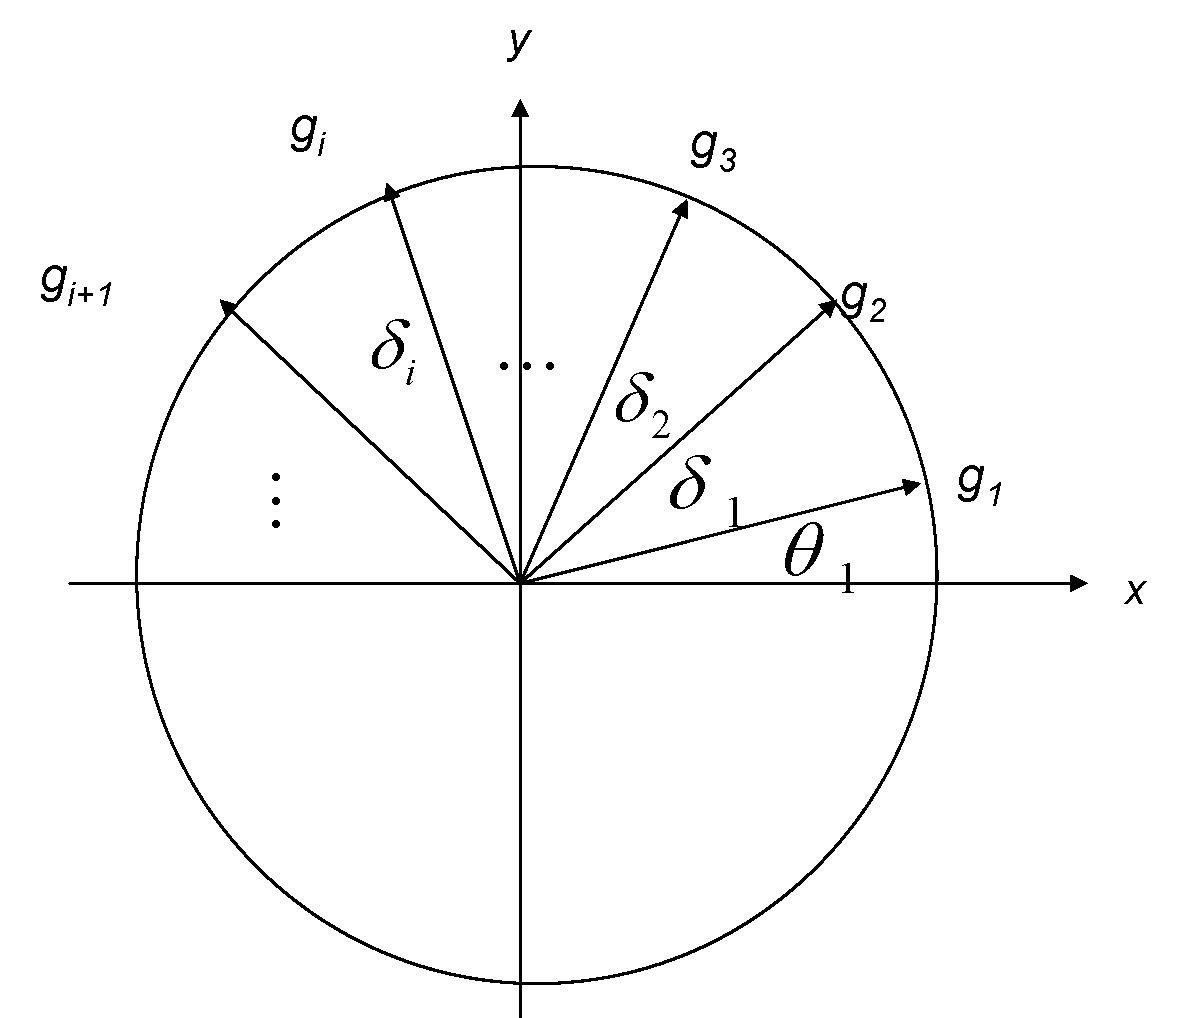
\includegraphics[width=2in]{opt_det_2erasures.png}
\caption{Adjust columns of $G$ such that $\theta_j =  \theta_1 + \sum_{k=1}^{j-1} \delta_k$.}
\label{spherical ball}
\end{figure}



The sub-matrix $G_{ij}$ (consisting of the column $i$ and $j$ of $G_{2 \times n}$) 
can be represented as 
\[ G_{ij}= \left( \begin{array}{cc}
\cos \theta_1 & \cos \theta_n \\
\sin \theta_1 & \sin \theta_n    \end{array} \right)\]

Therefore,
$$\det (G_{ij}) = \sin (\theta_j - \theta_i ) $$

\begin{eqnarray*}
\displaystyle \prod_{j>i} \det (G_{ij} ) 
&=& \displaystyle \prod_{j>i} \sin (\theta_j - \theta_i ) \\
&=& \displaystyle \prod_{j>i} \sin (\sum_{k=i}^{j-1} \delta_k) \\   
&=& \left( \sin \delta_1  \ldots  \sin \delta_{n-1}  \right)  \\ 
& & \left( \sin (\delta_1+\delta_2) \ldots \times \sin(\delta_{n-2}+\delta_{n-1})  \right)  \\
& &  \vdots \\
& & \sin (\delta_1 + \ldots +\delta_{n-1} ) \\ 
\end{eqnarray*}

Note that, when $x_i>0$
$$ \prod_{i=1}^n x_i \leq 
\left( \frac{ \sum_{i=1}^n x_i }{n} \right)^n.$$

When $x_1=x_2=\ldots=x_n=x$, the equality {\bf is achieved} and
$$\prod_{i=1}^n x_i = x^n.$$

Therefore, when $\delta_1=\delta_2=\ldots=\delta_{n-1}=\delta$,
for all $j=0,1,\ldots,n-2$, $\prod_{k=0}^{n-1-j} \sin (\sum_{t=0}^j \delta_{k+t})$
achieve their maximum $\sin^{n-1-j}((j+1)\delta)$ {\bf at the same time}. Therefore,
 $\prod_{j>i} \det (G_{ij} )$ achieves its maximum
\begin{eqnarray*}
\displaystyle \prod_{j>i} \det (G_{ij} )
&=& \sin^{n-1}\delta  \sin^{n-2} 2\delta 
 \ldots  \sin^1 ((n-1)\delta)
\end{eqnarray*}

Rearrange the right hand side of the above formula, we have
\begin{eqnarray*}
\displaystyle \prod_{j>i} \det (G_{ij} )
&=& ( \sin^{n-1}\delta   \times \sin^1 ((n-1)\delta)  \\
& & ( \sin^{n-2} 2\delta \times \sin^2((n-1)\delta)  \\
& & ( \sin^{n-3} 3\delta \times \sin^3((n-3)\delta)  \\
& & \vdots 
\end{eqnarray*}

When $\sin j \delta = \sin ((n-j)\delta)$, 
{\bf all} $\sin^{n-j} j\delta   \times \sin^j ((n-j)\delta)$
achieve, {\bf at the same time}, their maximum 
\begin{eqnarray*}
\left( \frac {(n-j) \sin j\delta + j \sin ((n-j)\delta)}{n} \right)^n
&=& (\sin j\delta)^n.
\end{eqnarray*}

Note that, when $\delta_1=\delta_2=\ldots=\delta_{n-1}=\delta$, 
$$
\pi = \delta_1 + \ldots + \delta_{n-1} + \delta_n=(n-1)\delta+\delta_n
$$
Therefore,
$$
\delta<\frac{\pi}{n-1}
$$
Therefore, $\sin j \delta = \sin ((n-j)\delta)$ implies
$$j \delta = \pi - (n-j)\delta$$
Therefore, implies
$$
\delta = \frac{\pi}{n}
$$
When $\delta_1=\delta_2=\ldots=\delta_{n-1}=\delta$,
$$
\delta_n=\pi-(\delta_1+\ldots+\delta_{n-1})=\frac{\pi}{n}.
$$

Therefore, when $\delta_1=\delta_2=\ldots=\delta_{n}=\frac{\pi}{n}$,
$\prod_i \det (G_i)$ achieve its maximum.

\end{proof}

\end{comment}




\begin{table*}[ht]
\caption{A generator matrix from Gaussian random matrices
with mean $0$ and standard deviation $1$.}
\begin{center}
\begin{tabular}{|r|r|r|r|r|r|r|r|r|r|}
\hline
$g_1$ & $g_2$ & $g_3$ & $g_4$ & $g_5$ & $g_6$ & $g_7$ & $g_8$ & $g_9$ &$g_{10}$ \\
\hline
0.0582    & -0.2290   & 0.1256     & -1.1022  & -2.6053  & -2.0564   & -0.0062   & -1.0216  & -0.9579   & -2.0886  \\
-1.6885   & 1.0350    & -1.2976    & 0.7591   & -0.8609  & -0.7067   & -1.3709   & -1.9139  & -0.7915   & 0.5943   \\
-1.2755   & -1.5523   & -0.8135    & 0.3585   & 0.0536   & -0.9256   & -0.4202   & -0.8843  & -0.8012   & 0.8242   \\
\hline
\end{tabular}
\end{center}
\end{table*}




\begin{table*}[ht]
\caption{A generator matrix from Grassmannian frames 
matrices.}
\begin{center}
\begin{tabular}{|r|r|r|r|r|r|r|r|r|r|}
\hline
$g_1$ & $g_2$ & $g_3$ & $g_4$ & $g_5$ & $g_6$ & $g_7$ & $g_8$ & $g_9$ &$g_{10}$ \\
\hline
    1.0000   & 0.6101    &0.6101   & 0.6101   & 0.6101  &  0.6101   & 0.6101   &      0 &        0   &      0  \\
         0   & 0.7923    &0.3961   &-0.3961   &-0.7923  & -0.3961   & 0.3961  &  0.8660 &  -0.8660  &       0  \\
         0   &      0    &0.6861   &0.6861    &     0   &-0.6861   &-0.6861   & 0.5000  &  0.5000   &-1.0000   \\
\hline
\end{tabular}
\end{center}
\end{table*}


\begin{table*}[ht]
\caption{An approximate generator matrix from numerically best real number codes.}
\begin{center}
\begin{tabular}{|r|r|r|r|r|r|r|r|r|r|}
\hline
$g_1$ & $g_2$ & $g_3$ & $g_4$ & $g_5$ & $g_6$ & $g_7$ & $g_8$ & $g_9$ &$g_{10}$ \\
\hline
   -0.5566    &0.1467   & 0.7247  &  0.9919  &  0.4631  & -0.6691 &   0.5614  & -0.2353  &  0.0686 &  -0.6749  \\
    0.8095    &0.7985   & 0.4905  &  0.1217  & -0.1332  & 0.2351  &  -0.6914  & -0.0325  &  0.9466 &  -0.5804  \\
    0.1871    &0.5839   & 0.4839  &  0.0365  &  0.8763  &  0.7050 &   0.4547  &  0.9714  & -0.3149 &   0.4556  \\
\hline
\end{tabular}
\end{center}
\end{table*}


\begin{table*}[ht]
\caption{The condition numbers of the worst ten $3\times3$ sub-matrices in different generator matrices.}
\begin{center}
\begin{tabular}{|l|l|l|l|l|l|l|l|l|l|l|}
\hline
Grass        &$0.1*10^{17}$ &$0.1*10^{17}$ &$0.3*10^{17}$ &$0.3*10^{17}$ &$0.3*10^{17}$  
             &$0.5*10^{17}$ &$0.7*10^{17}$ &$2*10^{17}$ &$2*10^{17}$ & Inf   \\
\hline
Rand         &111     &131.3   &145.1   &168.6   &199     &250.4   &366.7   &457.4   &786.7   &1891.1  \\
\hline
Best         &12.1652 &12.4318 &12.4371 &13.2190 &13.5483 &14.7503 &15.6580 &16.1104 &16.1609 &16.536 \\
\hline
\end{tabular}
\end{center}
\end{table*}



\section{Experimental Evaluation}


\subsection{Experimental Evaluation of the Numerical Stability}

The numerical properties of real number codes from Vandermonde matrices, Cauchy matrices, 
DCT matrices, DFT matrices, and Gaussian random matrices has been fully 
analyzed and compared in~\cite{zchen:random_codes}. Experimental results indicate that real 
number codes from  Gaussian random matrices
are much more stable than the other codes.

In this section, we will compare the numerically best codes with real number codes from 
Gaussian random matrices and Grassmannian frame matrices. 
When the number of erasures $m=2$, there are exact analytical expressions for the generator matrices 
of both the Grassmannian code and the numerically best code. The numerically best code
is the same as the Grassmannian code when $m=2$. They are both numerically optimal.
However, when the number of erasures $m\geq3$, the Grassmannian code is not optimal anymore.
Therefore, we focus on the comparison of the numerically stability of these codes for more than two erasures.



When the number of erasures $m\geq3$, most of time, there are no exact 
analytical expressions for the generator matrices of all three codes except for very 
few combinations of $m$ and $n$. Therefore, most of time, we have to use 
approximation codes in practice.

However, for $m=3$ and $n=10$, the mathematically optimal (without any computational approximation) 
Grassmanian (packing) codes are given in~\cite{conway:grassmannian}. It is a hexakis bi-antiprism. The columns of the 
corresponding generator matrix (i.e. the coordinates of the 10 points in three dimensional space)
are given in~\cite{grass}. Therefore, in this paper, we choose to compare the numerical stability of the three codes
to tolerate three failures in ten processors. Table 2 gives the corresponding generator matrix
of the Grassmannian code.



\begin{figure}
\centering
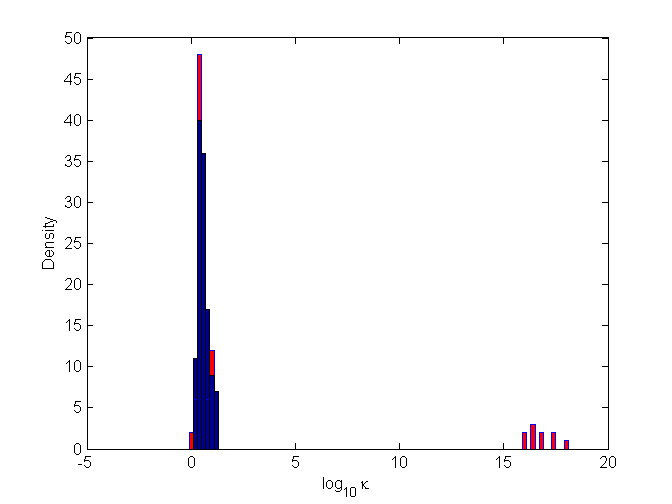
\includegraphics[width=3.6in]{grass_opt_b_120.png}
\caption{Condition number distribution for Grassmannian frame codes (red) and optimal codes (blue).}
\label{fig_sim}
\end{figure}

 
\begin{figure}
\centering
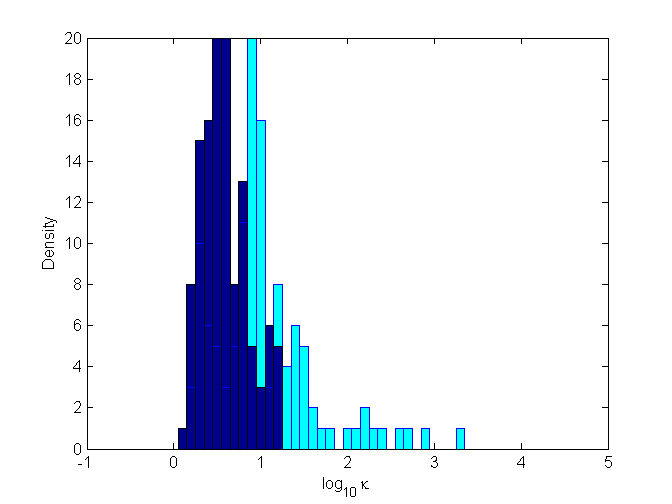
\includegraphics[width=3.6in]{rand_opt_b_120.png}
\caption{Condition number distribution for Gaussian random codes (cyan) and optimal codes (blue).}
\label{fig_sim}
\end{figure}


It is mathematically difficult to obtain analytical expressions for the numerically best codes
for three or more erasures. Therefore, for numerically best codes, we use the approximation 
codes computed by solving the unconstrained optimization problem 
in Section 4 to participate the comparison. 
Table 3 gives the corresponding generator matrix
of the numerically best code. 

Gaussian random codes are simple to generate using a pseudo Gaussian random number generator.
Table 1 gives the corresponding generator matrix of the Gaussian random code.
The matrix is generated using MATLAB.
Actually, this code is only a statistical approximation of the Gaussian random codes.
However, this is how we generate and use Gaussian random codes in practice.

As discussed in~\cite{golub89:matrix}, when solving a 
linear system of equations, a condition number of $10^k$ for the coefficient matrix
leads to a loss of accuracy of about $k$ decimal digits in the solution.
The coefficient matrix of the system of equations to be solved during recovery
can be any square sub-matrix (including minor) of the generator matrix.
Therefore, in what follows, we focus on comparing the condition numbers 
of the sub-matrices of all three generator matrices.

The size of the generator matrices is $3 \times 10$, therefore, the total number of $3 \times 3$ sub-matrices
in each generator matrix is 120. 






Table 4 gives the condition numbers of the 10 worst conditioned 
$3\times3$ sub-matrices in all three generator matrices.
Table 4 demonstrates that the condition numbers of all 
10 worst-conditioned $3\times3$ sub-matrices
of the numerically best code are much smaller than that of the other two codes.
Therefore, in the  worst case scenarios, the numerically best code is numerically much more stable
than both the Gaussian random code and the Grassmannian code.
Condition number is a property that associated with more than two columns of a matrix.
The Grassmannian codes maximizes only the minimum angle between any two columns of the generator matrix.
When the minimum angle between any two columns of the generator matrix achieves its global maximum,
it is still possible that three columns of a generator matrix are in the same plan, therefore,
the generator matrix contains a singular sub-matrix. This is exactly the reason why we get one singular sub-matrix
in the Grassmannian codes. Therefore, Grassmannian codes are generally {\bf NOT} optimal unless $m=2$ 
where a sub-matrix only contains $2$ columns.
The numerically best code minimizes the maximum condition numbers of all sub-matrices, therefore,
has a much better numerically stability in the worst case scenarios.

 


Figure 4 gives the distribution of all 120 condition numbers of all 120 $3\times3$ sub-matrices 
for both the Grassmannian code (red) and the numerically best code (blue).
Figure 4 demonstrates that the numerically best code are at least as good as the 
Grassmannian code in average cases.

Figure 5 shows the distribution of all 120 condition numbers of all 120 $3\times3$ sub-matrices 
for both Gaussian random code (cyan) and the numerically best code (blue). 
Figure 5 indicates that the numerically best code are much more stable than Gaussian random
codes in average cases.

\subsection{Experimental Evaluation of the Fault Tolerance Overhead}


\begin{figure}
\centering
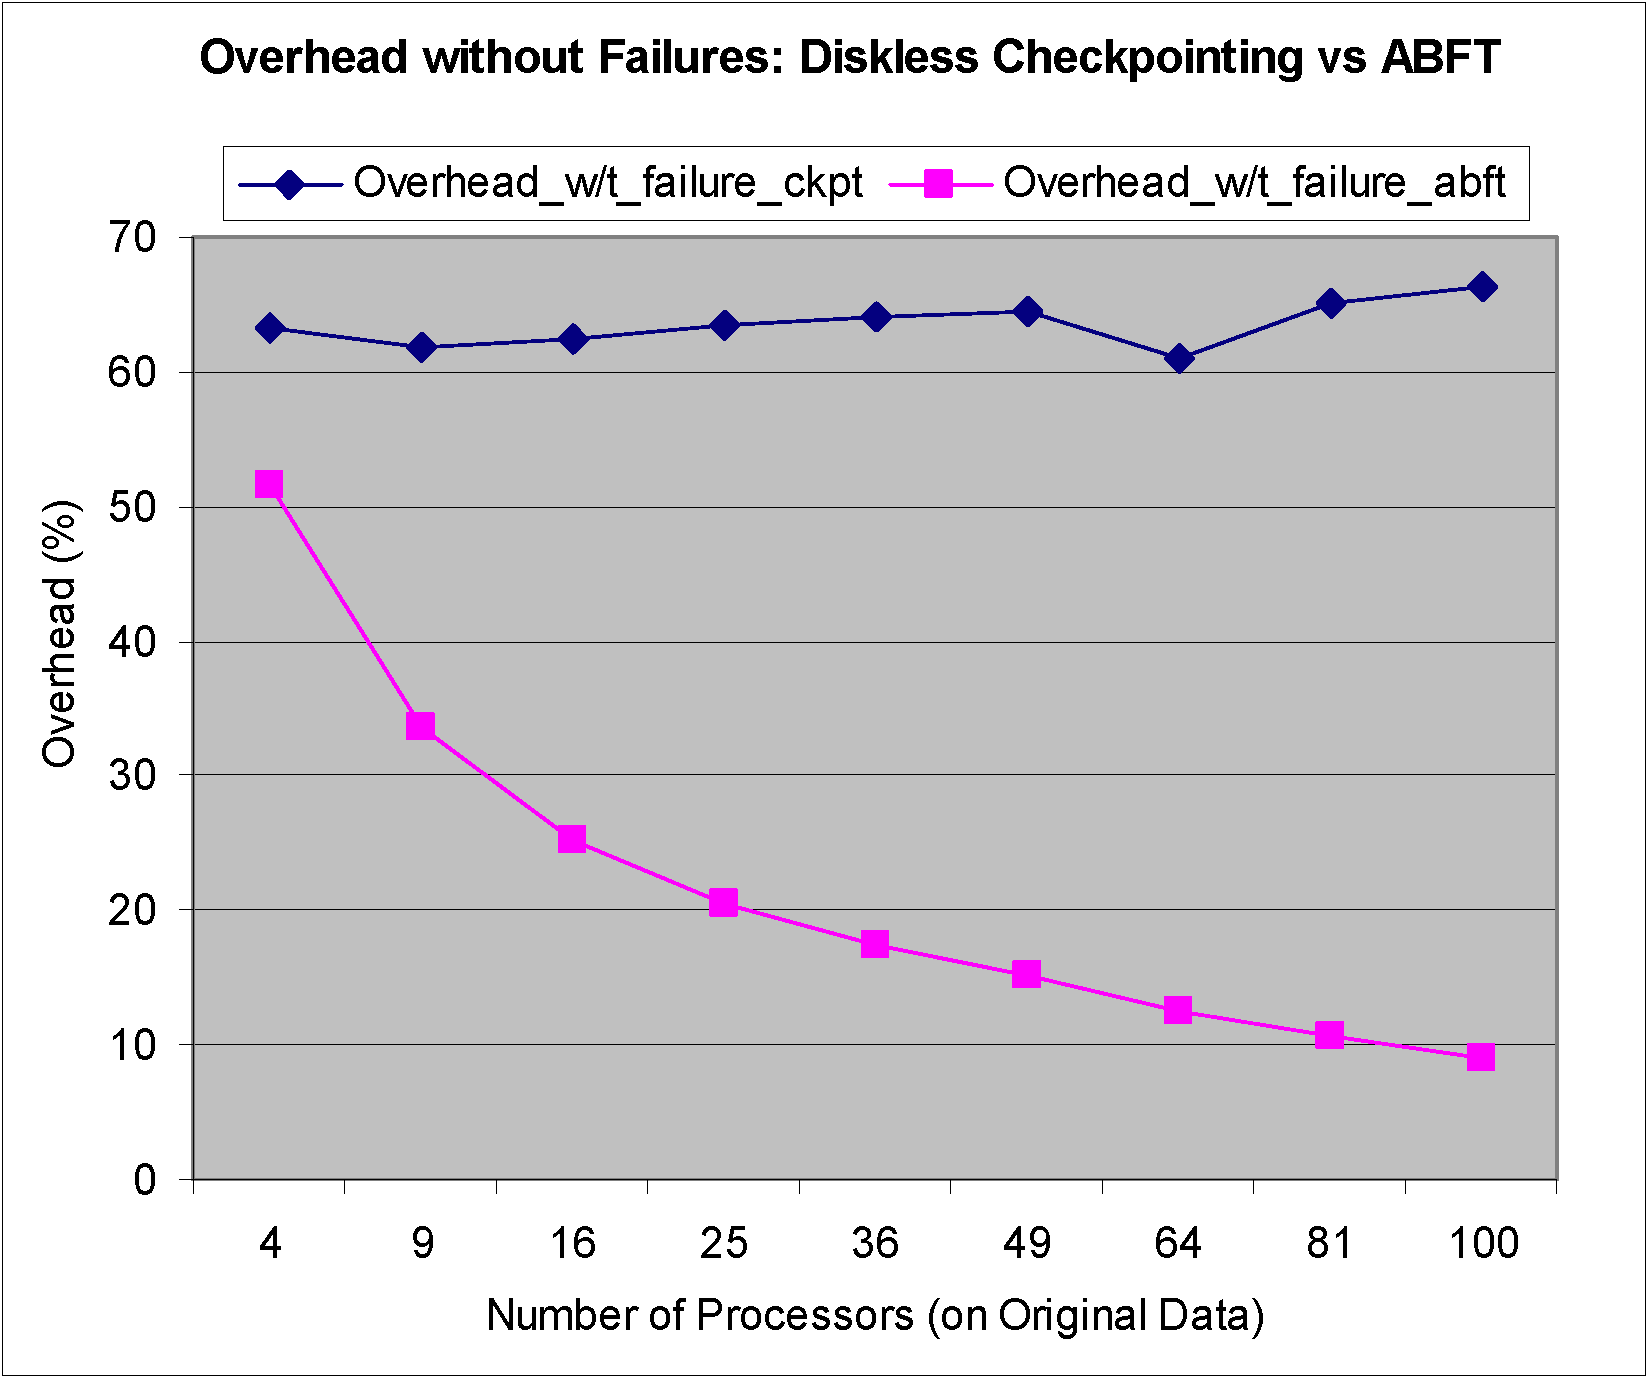
\includegraphics[width=3.2in]{overhead_mfailure_wt.png}
\caption{Fault tolerance overhead without failures: diskless checkpointing vs ABFT.}
\label{fig_sim}
\end{figure}

%\begin{comment}
\begin{figure}
\centering
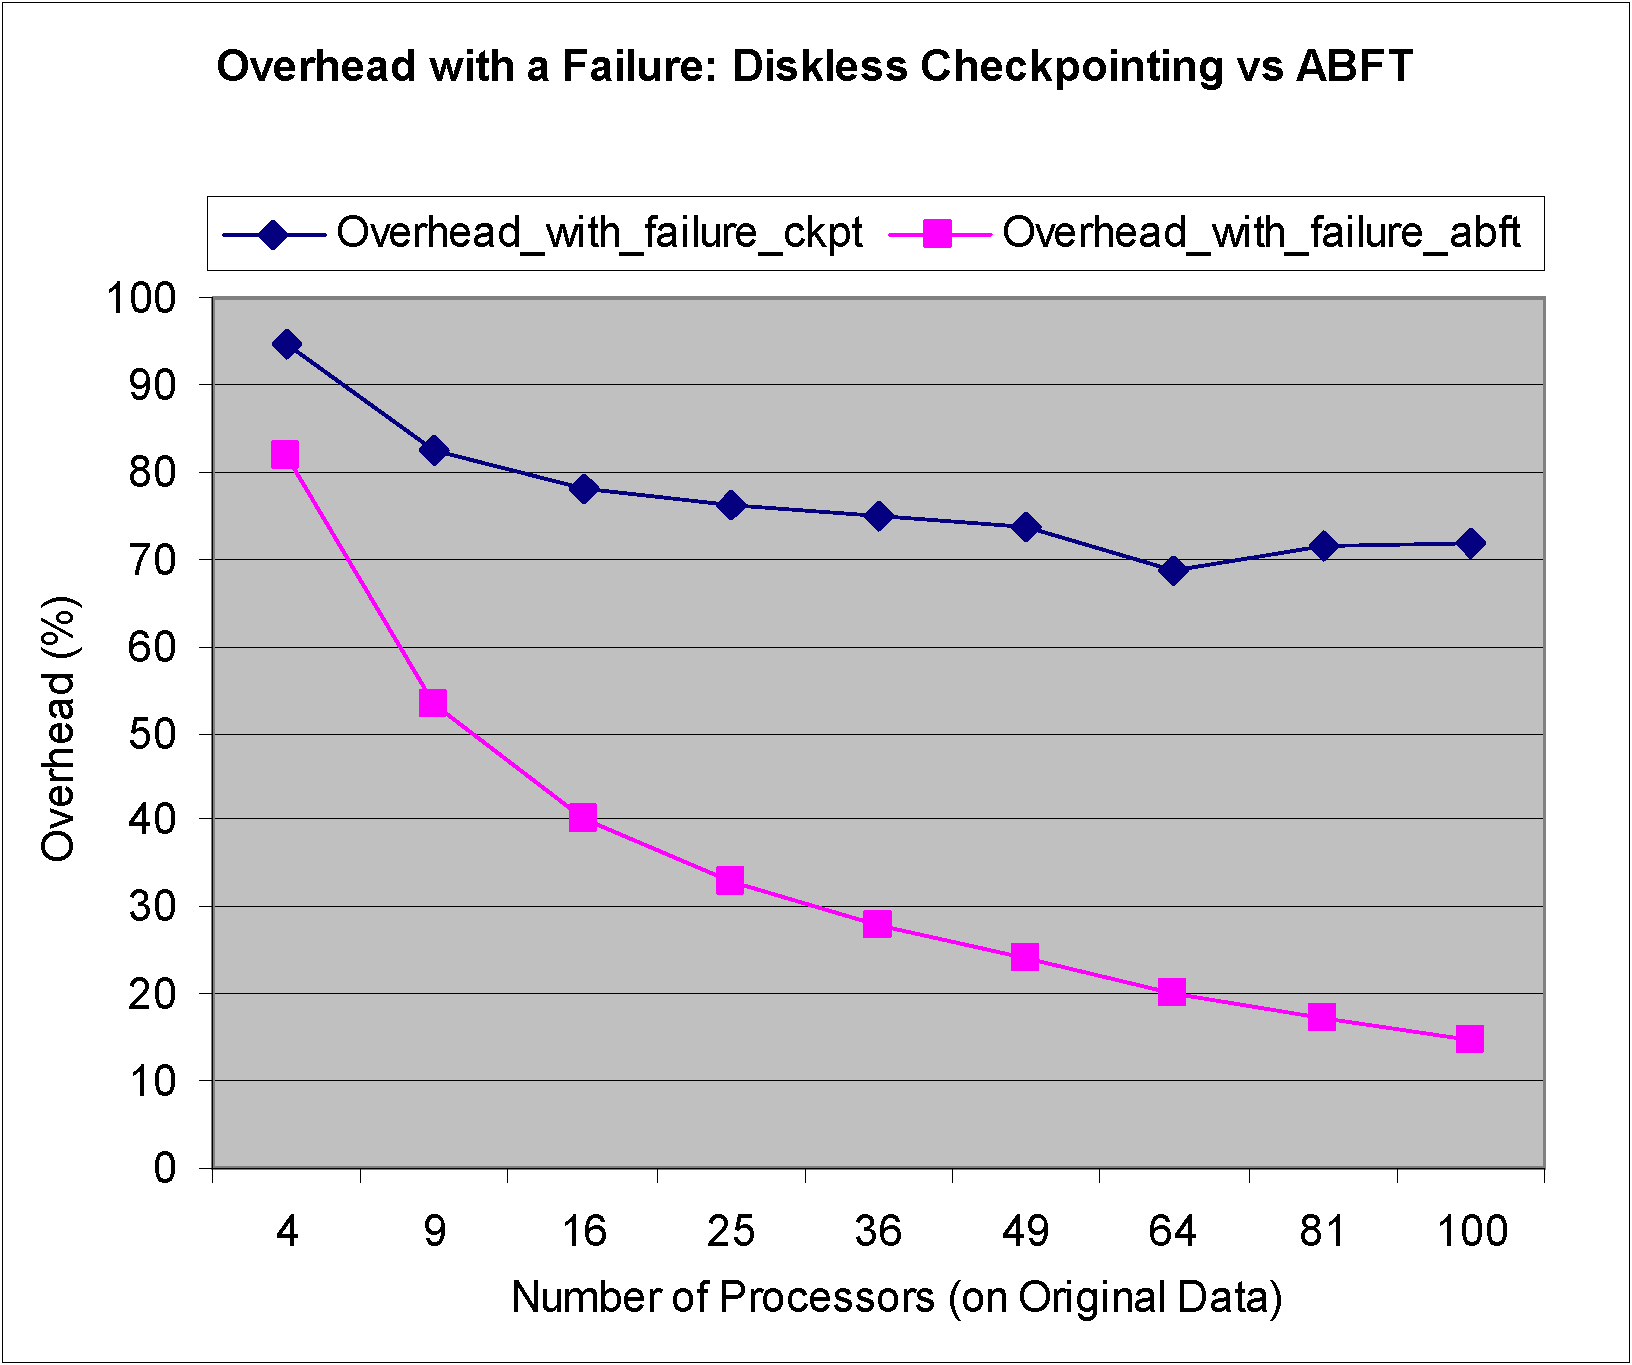
\includegraphics[width=3.2in]{overhead_mfailure_with.png}
\caption{Fault tolerance overhead with a failure of two processors at the same time: diskless checkpointing vs ABFT.}
\label{fig_sim}
\end{figure}
%\end{comment}


In this subsection, the fault tolerance overhead for the algorithm-based checkpoint-free approach 
is compared with the overhead of the triditional checkpoint based approach. Due to its high scalability and 
low overhead, diskless checkpointing has been chosen for the compariosn. 

The algorithm-based checkpoint-free scheme is configured
to tolerate a simultaneous failure of two processors using the optimal real number codes developed 
in Section 4. In the diskless checkpointing scheme, a Reed-Solomon based application level checkpoint scheme is used to 
tolerate a simultaneous failure of two processors. Two fault tolerant versions of the matrix-matrix multiplication
have been implemented using the two fault tolerance schemes. In the checkpoint scheme, the checkpoint interval
is about five minutes. At each checkpoint, three matrices are copied into the local memory of the computation
processes and encodings of these local checkpoints are saved into dedicated checkpoint processors.

Figure 6 compares the fault tolerance overhead of the two schemes when there are no actual failures occured.
As indicated by Figure 6, while the overhead of the disless checkpointing scheme is almost constant,
the overhead for the algorithm-based checkpoint-free approach decreases as the number of processors increases.
This is consistent with the theoretical analysis in~\cite{chen:abft}.


%\begin{comment}
In Figure 7,  we compare the fault tolerance overhead of the two schemes when there is 
a simultaneous failure of two processors in the middle of the computation.
Figure 7 demonstrates that the overhead of the diskless checkpointing scheme is still approximately constant.
But the overhead for the algorithm-based checkpoint-free approach decreases again as the number of processors increases.
The overhead for the algorithm-based checkpoint-free approach is much lower than the overhead of the 
diskless checkpointing scheme. Compared with diskless checkpointing,
the algorithm-based checkpoint-free approach has much better scalability.
%\end{comment}


\section{Conclusion}

In this paper, we present a class of numerically best real-number codes 
for fault tolerant matrix operations on large HPC systems. 
We give an analytical expression for the numerically best 
erasure correcting codes for two erasures and develop an approximation method to 
computationally approximate the numerically best codes for more than two erasures.
Experiment results demonstrate that our codes are numerically 
much more stable than existing codes. 

In the near future, we would like to explore better approximation methods to 
computationally approximate the numerically best codes 
for three or more erasures.



% Reminder: the "draftcls", not "draft", class option should be used if
% it is desired that the figures are to be displayed while in draft mode.

% An example of a floating figure using the graphicx package.
% Note that \label must occur AFTER (or within) \caption.
% For figures, \caption should occur after the \includegraphics.
%
%\begin{figure}
%\centering
%\includegraphics[width=2.5in]{myfigure.eps}
%\caption{Simulation Results}
%\label{fig_sim}
%\end{figure}


% An example of a double column floating figure using two subfigures.
% (The subfigure.sty package must be loaded for this to work.)
% The subfigure \label commands are set within each subfigure command, the
% \label for the overall fgure must come after \caption.
% \hfil must be used as a separator to get equal spacing
%
%\begin{figure*}
%\centerline{\subfigure[Case I]{\includegraphics[width=2.5in]{subfigcase1.eps}
%\label{fig_first_case}}
%\hfil
%\subfigure[Case II]{\includegraphics[width=2.5in]{subfigcase2.eps}
%\label{fig_second_case}}}
%\caption{Simulation results}
%\label{fig_sim}
%\end{figure*}



% An example of a floating table. Note that, for IEEE style tables, the
% \caption command should come BEFORE the table. Table text will default to
% \footnotesize as IEEE normally uses this smaller font for tables.
% The \label must come after \caption as always.
%
%\begin{table}
%% increase table row spacing, adjust to taste
%\renewcommand{\arraystretch}{1.3}
%\caption{An Example of a Table}
%\label{table_example}
%\centering
%% The array package and the MDW tools package offers better commands
%% for making tables than plain LaTeX2e's tabular which is used here.
%\begin{tabular}{|c||c|}
%\hline
%One & Two\\
%\hline
%Three & Four\\
%\hline
%\end{tabular}
%\end{table}


% if have a single appendix:
%\appendix[Proof of the Zonklar Equations]
% or
%\appendix  % for no appendix heading
% do not use \section anymore after \appendix, only \section*
% is possibly needed

% use appendices with more than one appendix
% then use \section to start each appendix
% you must declare a \section before using any
% \subsection or using \label (\appendices by itself
% starts a section numbered zero.)
%
% Use this command to get the appendices' numbers in "A", "B" instead of the
% default capitalized Roman numerals ("I", "II", etc.).
% However, the capital letter form may result in awkward subsection numbers
% (such as "A-A"). Capitalized Roman numerals are the default.
%\useRomanappendicesfalse
%


% you can choose not to have a title for an appendix
% if you want by leaving the argument blank
%\section{}


% use section* for acknowledgement
%\section*{Acknowledgment}
% optional entry into table of contents (if used)
%\addcontentsline{toc}{section}{Acknowledgment}

%The authors would like to thank... This work was supported by the IEEE.

% trigger a \newpage just before the given reference
% number - used to balance the columns on the last page
% adjust value as needed - may need to be readjusted if
% the document is modified later
%\IEEEtriggeratref{8}
% The "triggered" command can be changed if desired:
%\IEEEtriggercmd{\enlargethispage{-5in}}

% references section
% NOTE: BibTeX documentation can be easily obtained at:
% http://www.ctan.org/tex-archive/biblio/bibtex/contrib/doc/

% can use a bibliography generated by BibTeX as a .bbl file
% standard IEEE bibliography style from:
% http://www.ctan.org/tex-archive/macros/latex/contrib/supported/IEEEtran/
%\bibliographystyle{IEEEtran.bst}
% argument is your BibTeX string definitions and bibliography database(s)
%\bibliography{IEEEabrv,../bib/paper}
%
% <OR> manually copy in the resultant .bbl file
% set second argument of \begin to the number of references
% (used to reserve space for the reference number labels box)

\begin{thebibliography}{14}

%\bibitem{IEEEhowto:kopka}
%This is an example of a book reference
%H. Kopka and P.W. Daly, \emph{A Guide to {\LaTeX}}, third ed. Harlow, U.K.: Addison-Wesley, 1999.

%This is an example of a article reference
%A. Gefen, ``Simulations of Foot Stability During Gait Characteristic of Ankle Dorsiflexor Weakness
%in the Elderly,'' \emph{IEEE Trans. Neural Systems Rehabilitation Eng.,} vol. 9, no. 4, pp. 333-337, Dec. 2001.

%This is an example of a article from a conference proceeding
%T. Tuytelaars and L. van Gool ``Content-Based Image Retrieval Based on Local Affinely Invariant Regions,''
%\emph{Proc. Third Int'l Conf. Visual Information Systems,} pp. 493-500, 1999.

%Again, see the IEEEtrans_HOWTO.pdf for several more bibliographical examples. Also, more style examples
%can be seen at http://www.computer.org/author/style/transref.htm




\bibitem{top500}
Top 500 supercomputer sites. http://www.top500.org.

\bibitem{grass}
http://www.research.att.com/$\sim$njas/grass/dim3

\bibitem{anfinson:abft}
J.~Anfinson and F.~T.~Luk
\newblock A Linear Algebraic Model of Algorithm-Based Fault Tolerance.
\newblock {\em IEEE Transactions on Computers}, v.37 n.12, p.1599-1604, December 1988.

\bibitem{Banerjee90:abft}
P. Banerjee, J. T. Rahmeh, C. B. Stunkel, V. S. S. Nair, K. Roy, V. Balasubramanian, and J. A. Abraham
\newblock Algorithm-based fault tolerance on a hypercube multiprocessor.
\newblock {\em IEEE Transactions on Computers}, vol. C-39:1132--1145, 1990.

\bibitem{Balasubramanian90:abft}
V. Balasubramanian and P. Banerjee
\newblock Compiler-Assisted Synthesis of Algorithm-Based Checking in Multiprocessors.
\newblock {\em IEEE Transactions on Computers}, vol. C-39:436-446, 1990.

\bibitem{cappello:ft}
A. Bouteiller, P. Lemarinier, G. Krawezik, and F. Cappello.
\newblock Coordinated checkpoint versus message log for fault tolerant MPI.
\newblock {\em Procceedings of International Conference on Cluster Computing (Cluster 2003)}, 
Honk Hong, December, 2003.

\bibitem{dongarra96:scalapack}
L.~S. Blackford, J.~Choi, A.~Cleary, A.~Petitet, R.~C. Whaley, J.~Demmel,
  I.~Dhillon, K.~Stanley, J.~Dongarra, S.~Hammarling, G.~Henry, and D.~Walker.
\newblock {ScaLAPACK:} a portable linear algebra library for distributed memory
  computers - design issues and performance.
\newblock In {\em Supercomputing '96: Proceedings of the 1996 ACM/IEEE
  conference on Supercomputing (CDROM)}, page~5, 1996.


\bibitem{boley92:abft}
D.~L. Boley, R.~P. Brent, G.~H. Golub, and F.~T. Luk.
\newblock Algorithmic fault tolerance using the lanczos method.
\newblock {\em SIAM Journal on Matrix Analysis and Applications}, 13:312--332,
  1992.


\bibitem{tao:codes}
E. Candes, M. Rudelson, L. Tao, R. Vershynin
\newblock Error Correction via Linear Programming.
\newblock {\em Proc. 46th Annual IEEE Symposium on Foundations of Computer Science (FOCS05)}, 
IEEE, 2005.  pp. 295-308



\bibitem{zchen:random_codes_utk}
Z.~Chen and J.~Dongarra.
\newblock Numerically Stable Real-Number Codes Based on Random Matrices.
\newblock In {\em  ut-cs-04-526} June 9, 2004.

\bibitem{zchen:random_codes}
Z.~Chen and J.~Dongarra.
\newblock Numerically stable real number codes based on random matrices.
\newblock In {\em Proceeding of the 5th International Conference 
on Computational Science (ICCS2005)}, Atlanta, Georgia, USA, May 22-25, 2005. LNCS 3514, Springer-Verlag.

\bibitem{zchen:random_condition}
Z.~Chen and J.~Dongarra.
\newblock Condition Numbers of Gaussian Random Matrices.
\newblock {\em SIAM Journal on Matrix Analysis and Applications}, 
Volume 27, Number 3, Page 603-620, 2005.

\bibitem{chen:abft}
Z. Chen, and J. Dongarra.
\newblock Algorithm-Based Fault Tolerance for Fail-Stop Failures.
\newblock {\em IEEE Transactions on Parallel and Distributed Systems},
 Vol. 19, No. 12, December, 2008.

\bibitem{chen:scalable-checkpointing}
Z. Chen, and J. Dongarra.
\newblock Highly Scalable Self-Healing Algorithms for High Performance Scientific Computing.
\newblock {\em IEEE Transactions on Computers},
 July, 2009.

\bibitem{zchen05:diskless}
Z.~Chen, G.~E. Fagg, E.~Gabriel, J.~Langou, T.~Angskun, G.~Bosilca, and
  J.~Dongarra.
\newblock Fault tolerant high performance computing by a coding approach.
\newblock In {\em Proceedings of the ACM SIGPLAN Symposium on Principles and
  Practice of Parallel Programming, PPOPP 2005, June 14-17, 2005, Chicago, IL,
  USA}. ACM, 2005.


\bibitem{zchen05:ft-mpi}
Z.~Chen, G.~E. Fagg, E.~Gabriel, J.~Langou, T.~Angskun, G.~Bosilca, and
  J.~Dongarra.
\newblock Building Fault Survivable MPI Programs with FT-MPI Using Diskless Checkpointing.
\newblock In {\em University of Tennessee Computer Science Department Technical Report}. 
Technical Report UT-CS-04-540, 2004.


\bibitem{zchen:dissertation}
{Z. Chen}.
\newblock {\em {Scalable techniques for fault tolerant high performance computing}}.
\newblock {Ph.D. thesis, University of Tennessee}, {Knoxville, TN, USA}, {2006}.



\bibitem{conway:grassmannian}
J. H. Conway, R. H. Hardin and N. J. A. Sloane
\newblock Packing Lines, Planes, etc.: Packings in Grassmannian Spaces.
\newblock {\em Experimental Mathematics}, Vol. 5, No. 2, 1996



\bibitem{donoho:L1_minimization}
D. L. Donoho
\newblock For most large undetermined systems of linear
equations the minimal `1-norm near-solution is also the
sparsest near-solution.
\newblock {\em Communications on Pure and Applied Mathematics}, 
Volume 59 Issue 6, Pages 797 - 829


\bibitem{donoho:compressed}
D. L. Donoho
\newblock Compressed sensing.
\newblock {\em IEEE Trans. on Information Theory}, 
52(4), pp. 1289 - 1306, April 2006



\bibitem{edelman88:randm}
A.~Edelman.
\newblock Eigenvalues and condition numbers of random matrices.
\newblock {\em SIAM J. Matrix Anal. Appl.}, 9(4):543--560, 1988.




\bibitem{Ferreira00} 
Ferreira, P.
\newblock Stability issues in error control coding in
complex field, interpolation, and frame bounds.
\newblock {\em IEEE Signal Processing Letters}, 
vol.7 No.3,(2000) pp.57-59.

\bibitem{Ferreira03} 
Ferreira, P., Vieira, J.  
\newblock Stable DFT codes and frames,
\newblock {\em IEEE Signal Processing Letters}, vol.10 No.2,(2003) pp.50-53.


\bibitem{goyal: erasure}
V. K. Goyal and J. Kovacevic
\newblock Quantized Frame Expansions with Erasures
\newblock {\em Applied and Computational Harmonic Analysis}  vol.10, 203 233 (2001)


\bibitem{gunnels:abft}
J. Gunnels, R. van de Geijn, D. Katz, E. Quintana-Ort 
\newblock Fault-Tolerant High-Performance Matrix Multiplication: Theory and Practice
\newblock {\em Proceedings of the 2001 International Conference on Dependable Systems and Networks (DSN'01) }, Washington, DC,  USA, 2001.


\bibitem{geijn:plapack}
P. Alpatov, G. Baker, C. Edwards, J. Gunnels, G. Morrow
J. Overfelt, R. van de Geijn, and J. Wu.
\newblock PLAPACK: Parallel Linear Algebra Libraries Design Overview
\newblock {\em Proc. of the SC97 Conference}, ACM, San Diego, CA, 1997.

\bibitem{golub89:matrix}
{G. H. Golub and C. F. Van Loan}.
\newblock {\em {Matrix Computations}}.
\newblock {The John Hopkins University Press}, {}, {1989}.

\bibitem{hadjicostis:coding}
C. N. Hadjicostis.
\newblock {\em Coding Approaches to Fault Tolerance in Combinational and Dynamic Systems},
Kluwer Academic Publishers, 2002.  


\bibitem{huang84:abft}
K.-H. Huang and J.~A. Abraham.
\newblock Algorithm-based fault tolerance for matrix operations.
\newblock {\em IEEE Transactions on Computers}, vol. C-33:518--528, 1984.

\bibitem{kim96:abft}
Y.~Kim.
\newblock {\em Fault Tolerant Matrix Operations for Parallel and Distributed
  Systems.}
\newblock {P}h.{D}. dissertation, University of Tennessee, Knoxville, June


\bibitem{knuth:random}
D. E. Knuth.
\newblock {\em The Art of Computer Programming}, 
Addison-Wesley Professional, 2 edition, October 15, 1998.


\bibitem{langou:ft}
J. Langou, Z. Chen, G. Bosilca, and J. Dongarra.
\newblock Recovery Patterns for Iterative Methods in a Parallel Unstable Environment
\newblock {\em SIAM Journal on Scientific Computing}, 30(1):102-116, 2007.

\bibitem{luk84:abft}
F.~T.~Luk and H.~Park
\newblock An analysis of algorithm-based fault tolerance techniques.
\newblock {\em SPIE Adv. Alg. and Arch. for Signal Proc.}, vol. 696, 1986, pp. 222-228.


\bibitem{marshall:realcodes}
T. Marshall
\newblock Coding of Real-Number Sequences for Error Correction: A Digital Signal Processing Problem.
\newblock {\em IEEE Journal on Selected Areas in Communications}, 
Volume 2, Issue 2, Mar 1984 Page(s): 381 - 392


\bibitem{Nair90} 
Nair, S. S. and Abraham, J. A.:
Real-number codes for fault-tolerant
matrix operations on processor arrays, IEEE Transactions on Computers, vol. C-39,(1990) pp.300-304.


\bibitem{plank:abft}
J.~S.~Plank, Y.~Kim, and J.~Dongarra.
\newblock Fault Tolerant Matrix Operations for Networks of Workstations Using Diskless Checkpointing.
\newblock {\em IEEE Journal of Parallel and Distributed Computing}, 43, 125-138 (1997).


\bibitem{plank:dc}
J.~S. Plank, K.~Li, and M.~A. Puening.
\newblock Diskless checkpointing.
\newblock {\em IEEE Trans. Parallel Distrib. Syst.}, 9(10):972--986, 1998.



\vfill \eject



\bibitem{plank97:rscode}
J.~S. Plank.
\newblock A tutorial on {R}eed-{S}olomon coding for fault-tolerance in
  {RAID}-like systems.
\newblock {\em Software -- Practice \& Experience}, 27(9):995--1012, September
  1997.




\bibitem{redinbo2:abft}
J. L. Sung and G. R. Redinbo.
\newblock Algorithm-Based Fault Tolerant Synthesis for Linear Operations.
\newblock {\em IEEE Transactions on Computers}, 
Volume 45 ,  Issue 4, April 1996.

\bibitem{redinbo:abft}
G. Robert Redinbo.
\newblock Generalized Algorithm-Based Fault Tolerance: Error Correction via Kalman Estimation.
\newblock {\em IEEE Transactions on Computers}, 
Volume 47,  Issue 6,June, 1998.

\bibitem{stellner:cocheck}
G. Stellner.
\newblock CoCheck: Checkpointing and process migration for MPI.
\newblock {\em Proceedings of the 10th International Parallel Processing Symposium (IPPS'96)}, 
Honolulu, Hawaii, April, 1996.


\bibitem{smale:unsolved}
S. Smale.
\newblock Mathematical Problems for the Next Century.
\newblock {\em Mathematics: Frontiers and Perspectives}, 
Ed. V. Arnold, M. Atiyah, P. Lax, and B. Mazur, Providence, RI: Amer. Math. Soc., 2000. 


\bibitem{strohmer03:grassmannian}
T.~Strohmer and R.~W.~Heath
\newblock Grassmannian frames with applications to coding and communication 
\newblock {\em Applied and Computational Harmonic Analysis}, Volume 14, Issue 3, Pages 257-275, May 2003.

\bibitem{gibson1:failure}
B. Schroeder and G. A. Gibson.
\newblock A large-scale study of failures in high-performance computing systems.
\newblock {\em Proceedings of the International Conference on Dependable Systems and Networks (DSN2006)}, Philadelphia, PA, USA,  June 25-28, 2006.

\bibitem{gibson2:failure}
B. Schroeder and G. A. Gibson.
\newblock Understanding Failures in Petascale Computers.
\newblock {\em Journal of Physics: Conference Series}, 78, 2007.

\bibitem{gibson3:failure}
G. A. Gibson, B. Schroeder, and J. Digney.
\newblock Failure Tolerance in Petascale Computers.
\newblock {\em CTWatchQuarterly}, Volume 3, Number 4, November 2007.



\bibitem{wang:blcr}
C.~Wang, F.~Mueller, C.~Engelmann, and S.~Scot.
\newblock Job Pause Service under LAM/MPI+BLCR for Transparent Fault Tolerance.
\newblock In {\em Proceedings of the 21st IEEE International Parallel and 
Distributed Processing Symposium, March, 2007, Long Beach, CA, USA}.

\bibitem{wang:abft}
S. J. Wang and N.K.  Jha.
\newblock Algorithm-Based Fault Tolerance for FFT Networks.
\newblock {\em IEEE Transactions on Computers}, 
Volume 43,  Issue 7,July, 1994.



\end{thebibliography}



% biography section
%
% If you had an eps/pdf photo file (graphicx package needed)
% the extra braces prevent the LaTeX parser from getting confused
% when it sees the complicated \includegraphics command within an
% optional argument. You can create your own macro to make things
% simpler here.
%\begin{biography}[{\includegraphics[width=1in,height=1.25in,clip,keepaspectratio]{mshell.eps}}]{Michael Shell}
% or if you just want to reserve a space for a photo:

%\begin{biography}{Michael Shell}
%Biography text here.
%\end{biography}

% if you will not have a photo
%\begin{biographynophoto}{John Doe}
%Biography text here.
%\end{biographynophoto}

% insert where needed to balance the two columns on the last page
%\newpage

%\begin{biographynophoto}{Jane Doe}
%Biography text here.
%\end{biographynophoto}

% You can push biographies down or up by placing
% a \vfill before or after them. The appropriate
% use of \vfill depends on what kind of text is
% on the last page and whether or not the columns
% are being equalized.

%\vfill

% Can be used to pull up biographies so that the bottom of the last one
% is flush with the other column.
%\enlargethispage{-5in}

% that's all folks
\end{document}


